
\documentclass[11pt, draft, oneside]{fithesis2}

%% Basic packages
\usepackage[czech]{babel}
\usepackage[utf8]{inputenc}
\usepackage{cmap}
\usepackage[T1]{fontenc}
\usepackage{float}
%\usepackage{lmodern}
\usepackage{graphicx}
\DeclareGraphicsExtensions{.pdf,.png,.jpg}
\graphicspath{ {./images/} }
%% Package used in architecture document
\usepackage{tikz}
\usetikzlibrary{%
  arrows,%
  fit,%
  patterns,%
  shapes.geometric,%
  shapes.misc,%
  shapes.symbols,%
  shapes.arrows,%
  shapes.callouts,%
  shapes.multipart,%
  shapes.gates.logic.US,%
  shapes.gates.logic.IEC,%
  er,%
  backgrounds,%
  chains,%
  trees,%
  matrix,%
  calendar,%
  folding,%
  fadings,%
  through,%
  positioning,%
  scopes,%
  decorations.fractals,%
  decorations.shapes,%
  decorations.text,%
  decorations.pathmorphing,%
  decorations.pathreplacing,%
  decorations.footprints,%
  decorations.markings,%
  shadows}  


%% Additional packages for colors, advanced
%% formatting options, etc.
\usepackage{color}
\usepackage{microtype}
\usepackage{url}
\usepackage{cslatexquotes}
\usepackage{fancyvrb}
\usepackage[small,bf]{caption}
\usepackage[numbers]{natbib} 
%%\usepackage[plainpages=false,pdfpagelabels,unicode]{hyperref}
\usepackage{amssymb} % required by correction notes
\usepackage{hyperref}
%\usepackage[all]{hypcap} - problem s nutnosti mit caption u figure
\usepackage{xspace}
\usepackage{paralist} % CompactItem
\usepackage{fancyvrb} % Verbatim zarovnany na stred
%\usepackage[paper=a4paper,top=2.5cm,bottom=2.5cm,left=2.5cm,right=2.5cm,foot=1cm]{geometry} % Nastavení rozměrů stránky

\newcommand{\polozka}[1]{\item {\bf #1}\xspace}
\newcommand{\paragraphNewLine}[1]{\paragraph*{#1}\mbox{}\\}

\usepackage{listings} % Code examples
%% Nove caption u listingu kódu
\renewcommand\lstlistingname{XML schéma} 
%% XML Listing - http://tex.stackexchange.com/questions/10255/xml-syntax-highlighting
\usepackage{color}
\usepackage{textcomp}
\definecolor{gray}{rgb}{0.4,0.4,0.4}
\definecolor{darkblue}{rgb}{0.0,0.0,0.6}
\definecolor{cyan}{rgb}{0.0,0.6,0.6}
\definecolor{palatinatepurple}{rgb}{0.41, 0.16, 0.38}

\lstset{
	captionpos=b, % Caption je pod ukazkou kodu
  basicstyle=\ttfamily\scriptsize,
  columns=fullflexible,
  showstringspaces=false,
  commentstyle=\color{gray}\upshape,
	breaklines=true
}

\lstdefinelanguage{XML}
{
%% XML
%%	comment=[l]{##}
  morestring=[b]",
  morestring=[s]{>}{<},
  morecomment=[s]{<?}{?>},
  stringstyle=\color{palatinatepurple},
  identifierstyle=\color{darkblue},
  keywordstyle=\color{cyan},
  morekeywords={xmlns, version, type, element, attribute, default namespace}% list your attributes here
}

%% UML for TIKZ
\usepackage{tikz-uml}

\widowpenalty 10000
\clubpenalty 10000

% Komentáře pomocí \ovnote{text}
\newcounter{ovNoteCounter}
\newcommand{\ovnote}[1]{{\scriptsize\color{red} $\divideontimes$ \refstepcounter{ovNoteCounter}\textsf{[OV]$_{\arabic{ovNoteCounter}}$:{#1}}}}

%% Fix long URLs in DVIs
\usepackage{ifpdf}

\ifpdf
\else
  \usepackage{breakurl}
\fi

%% Packages used to generate various lists
\usepackage{makeidx}
\makeindex

\usepackage[xindy]{glossaries}
\makeglossary

%% Use STAR and CIRCLE signs for nested
%% itemized lists
\renewcommand{\labelitemii}{$\star$}
\renewcommand{\labelitemiii}{$\circ$}
\newcommand{\ProjectName}{\mbox{BBMRI\_CZ}\xspace}

%% Title page information
\thesistitle{Návrh a~implementace centrálního indexu \ProjectName}
\thesissubtitle{Diplomová práce}
\thesisstudent{Ondřej Vojtíšek}
\thesiswoman{false} %% Important when using Slovak or Czech lang
\thesisfaculty{fi}  %% {fi, eco, law, sci, fsps, phil, ped, med, fss}
\thesislang{cs}     %% {en, sk, cs}
\thesisyear{Jaro 2014}
\thesisadvisor{RNDr. Petr Holub, Ph.D.}



%% Beginning of the document
\begin{document}


%% Nastavení zalamování slov
\hyphenation{in-fra-struk-tu-ra in-fra-struk-tu-ry we-bo-vé-ho iden-ti-fi-ká-toru žá-dan-ky
me-ta-s-tá-zy ali-kvo-tu}

%% Front page with a logo and basic thesis information
\FrontMatter
\ThesisTitlePage

%% Thesis declaration (required)
\begin{ThesisDeclaration}
  \DeclarationText
  \AdvisorName
\end{ThesisDeclaration}

%% Thanks
\begin{ThesisThanks}
Na tomto místě bych rád poděkoval vedoucímu mé práce RNDr. Petru Holubovi, PhD., za vedení a~množství rad jak odborných, tak i~zcela neinformatických. Vážím si toho, že mi bylo umožněno pracovat na reálném a~smysluplném projektu, přestože jsem do něho vstupoval takřka jako \textit{tabula rasa}.

Mé poděkování též patří Mgr. Janu Sochorovi za velkou pomoc s~pronikáním do tajů webového vývoje. 
V~neposlední řadě bych rád poděkoval kolegům a~partnerům zapojeným do projektu za jejich trpělivost a~ochotu pomoci. Z~mnoha osob bych zde rád jmenoval alespoň Ing. Danu Knoflíčkovou z~Masarykova onkologického ústavu. 
\end{ThesisThanks}




% ------------------------------------------------------------------------   
% ------------------------------------------------------------------------   
%% Shrnutí
% ------------------------------------------------------------------------   
\chapter*{Shrnutí}
Diplomová práce se zaměřuje na analýzu, návrh a~implementaci informatické infrastruktury pro projekt \ProjectName. Projekt se zabývá podporou výzkumu nádorových onemocnění v~České republice. Informatická infrastr\-uktura, má figurovat jako nástroj usnadňující používat pro výzkum biologický materiál jiných institucí. Práce obsahuje charakteristiku systémů, se kterými bude aplikace spolupracovat, a~představuje řešení splňující požadavky projektu.

\vspace{4em} 
\noindent {\Large\textbf{Klíčová slova}} \\ \\ 
\noindent BBMRI, \ProjectName, BBMRI-ERIC, Java EE, J2EE, Stripes, Spring, Hibernate, biobanking

%% Beginning of the thesis itself
\MainMatter

%% TOC (required)
\tableofcontents



% ------------------------------------------------------------------------   
% ------------------------------------------------------------------------      
% Uvod
% ------------------------------------------------------------------------   
\chapter{Úvod}
Schopnost státu poskytovat zdravotní péči občanům vyplývá z~možností, jaké poskytuje vybudovaná infrastruktura zdravotnických zařízení. Pro pacienta je klíčové jakou vzdálenost musí urazit, aby se mu dostalo potřebné léčby v~požadované kvalitě. Aby byla síť zdravotnických zařízení dostatečně hustá a~pacient to měl blízko ke specialistovi s~potřebnou znalostí a~vybavením, je definován požadavek na dojezdovou dobu vyjadřující lokální dostupnost hrazených služeb\footnote{Nařízení vlády č. 307/2012 Sb., o~místní a~časové dostupnosti zdravotních služeb.}. V~zájmu státu je tedy vybudovat, informatickým slovníkem řečeno, distribuovanou infrastrukturu, která zajistí požadovanou dostupnost služeb pro co nejvíce obyvatel. 

Popsaná struktura ale není příliš vhodná pro výzkum v~oblasti medicíny. Diagnózy stejných nemocí jsou rozesety napříč nemocnicemi v~celé republice tak, že mnohdy není v~rámci pracoviště dostatek potřebných dat pro stanovení relevantních závěrů.

Část dat je sice dostupná v~rámci ÚZISu (Ústav zdravotnických informací a~statistiky) ČR, NZISu (Národní zdravotnický informační systém), ve specializovaných registrech zřizovaných v~rámci NZISu (v~kontextu práce je zajímavý především NOR - Národní onkologický registr) nebo formou záznamů zdravotnických pojišťoven, ale ani to neřeší všechno. Pro výzkum může být nezbytné mít data v~jiném formátu, s~jinou granularitou apod., než jaké jsou zpravidla k~dispozici v~uvedených institucích.  

Pro realizaci výzkumu je často jedinou cestou navázat přímou spolupráci mezi nemocnicemi (resp. především fakultními), jakožto primárními zdroji dat. Umožnění takové formy spolupráce ale není jednoduché díky množství formálních, legislativních i~čistě praktických překážek. Pacientská data jsou považována za citlivé osobní údaje\footnote{Zákon č.101/2000 Sb., § 4, písm. b }, takže jejich použití pro výzkum je možné jen za konkrétních podmínek stanovených zákonem. Základním požadavkem je mít souhlas pacienta, který opravňuje k~použití dat vzniklých při léčbě pacienta pro jiné než klinické účely. V~případě vzácnějších chorob je ale nutné získat data z~většího počtu zařízení. V~tomto kroku může nastat problém ve sběru dat. Nemocnice, i~přes relativní monopol SW firmy \textit{STAPRO s.r.o.}, nepracují vždy se stejnou strukturou dat ve svých informačních systémech. Často jsou používány (především ve výzkumné experimentální oblasti) vlastní proprietární nástroje, číselníky unikátní jen pro dané pracoviště, a~množství informací je ukládáno v~nestrukturované podobě, kterou není možné automatizovaně zpracovávat nástroji, jaké poskytuje informatika nebo statistika. Dle vlastních zkušeností autora často chybí lidé s~medicínskými znalostmi a~zároveň s~abstraktním nadhledem, kteří by byli schopni popsat data a~jejich vztahy. Pro čistokrevné informatiky tak není vůbec snadné do této oblasti proniknout a~sestrojit datový model na základě komunikace s~odborníky. Pokud už někdo z~doktorů-výzkumníků je schopen informace strukturovat, tak si nasbíraná data pečlivě střeží doslova jako \uv{rodinné stříbro} a~odborné veřejnosti je poskytne nejdříve v~podobě přílohy k~již publikovanému výzkumu. To jsou jen některé z~překážek, se kterými se výzkum v~oblasti medicíny potýká.

Projekt, jehož součástí je aplikace popsaná touto prací si klade za cíl vybudování infrastruktury umožňující spolupráci napříč výzkumnými pracovišti zabývajícími se onkologií. 

Jelikož se téma práce týká reálného projektu, kladl si autor práce při psaní za cíl sepsat dokument, který by uchoval co nejvíce informací a~know-how pro případnou změnu vývojáře systému. Snahou bylo především popsat argumenty, které vedly ke stávajícímu použitému řešení. Z~hlediska implementace pak popsat a~vysvětlit části, které by nemusely být zcela intuitivní.

Tato práce se nedrží úplně typické struktury diplomových prací v~tom smyslu, že se v~ní nenachází pevná linie oddělující teoretickou a~praktickou část. Podobně zde neexistuje ani ostrá hranice mezi tím, co bylo prací autora a~co je pouze shrnutí existujících skutečností. V~kapitole~\ref{chapter:analysis} je popsán projekt a~jeho cíle. Dále jsou popsány požadavky na systém. Část těchto požadavků není dílem autora této práce a~je rešerší dokumentu z~roku 2011 viz~\cite{ARCH_2011_12_29}. Některé uvedené skutečnosti jsou naopak výsledkem jednání autora a~také výsledkem konzultací prototypu aplikace. Část těchto skutečností je uvedena již v~dokumentu~\cite{ARCH_2014_1_25}. Autor se chtěl záměrně vyhnout \uv{dramatizaci} procesu vývoje jednání a~tak jsou většinou popisována jen výsledná řešení. V~některých konkrétních případech nicméně autor považoval za přínosné, aby bylo popsáno nebo lehce nastíněno, co k~rozhodnutím vedlo a~jaké byly nezvolené alternativy.

Kapitola~\ref{chapter:proposal} obsahuje popis toho, jakým způsobem byly požadavky na systém převedeny do řeči OOP (objektově orientované programování). Poslední \ref{chapter:implementation}.~kapitola obsahuje stručný popis použitých technologii a~popis, jakým způsobem byly některé vybrané části kódu implementovány. Pro implementaci byly použity standardní a~mezi programátory Java EE aplikací známé nástroje. Jejich popisu je tedy věnován pouze malý prostor.









% ------------------------------------------------------------------------ 
% ------------------------------------------------------------------------      
% Analyza
% ------------------------------------------------------------------------   
\chapter{Analýza}\label{chapter:analysis}

% ------------------------------------------------------------------------   
% ------------------------------------------------------------------------   
\section{Popis projektu \ProjectName}\label{chapter:analysis:section:projectDescription}
BBMRI (Biobanking and Biomolecular Resources Research Infrastructure) je celoevropský projekt, jehož cílem je vytvořit jednotnou infrastrukturu nad fakultními nemocnicemi, biobankami\footnote{Biobankou je v~kontextu práce myšleno pracoviště dlouhodobě uchovávající biologický materiál.} a~dalšími výzkumnými pracovišti umožňující výměnu dat a~biologického materiálu mezi institucemi pro potřeby výzkumu. Dílčími cíly projektu je vyřešení legislativních otázek, týkajících se nakládání s~biologickým materiálem, standardizace uchovávání vzorků, sjednocení pohledu na strukturu ukládaných dat a~další kroky nutné pro usnadnění výzkumu a~spolupráce napříč pracovišti a~zapojenými státy. Project výzkumné infrastruktury BBMRI je implementován v~rámci konsorcia ERIC (proto je od roku 2013 projekt označován zkratkou BBMRI-ERIC).

\ProjectName je česká odnož projektu BBMRI, jejímž cílem je vytvořit českou síť biobank přidružených k~lékařským fakultám, které budou dlouhodobě uchovávat biologický materiál pacientů nádorových onemocnění. Cílem projektu je, stejně jako v~případě celoevropského BBMRI, prostřednictvím výměny uchovávaných vzorků a~souvisejících informací mezi institucemi zlepšit prostředí pro výzkum nádorových onemocnění. V~dlouhodobém horizontu je cílem zapojit vznikající infrastrukturu \ProjectName do celoevropské infrastruktury BBMRI-ERIC. 

Koordinátorem projektu je Masarykův onkologický ústav (dále MOÚ). Technologickým partnerem na projektu je centrum CERIT-SC. To má na starosti vybudování a~správu informatické infrastruktury – indexu a~monitorovací služby \ProjectName. Návrhu a~implementaci těchto služeb se věnuje tato práce.

% ------------------------------------------------------------------------   
% ------------------------------------------------------------------------   
\section{Indexová služba}\label{chapter:analysis:section:index}
Pacientská data jsou uložena v~nemocničním informačním systému (dále jen NIS) a~obsahují veškeré záznamy o~průběhu léčby pacienta a~o~souvisejících vyšetřeních, tj. operace, laboratorní analýzy, kontroly a~další záznamy. Indexová služba \ProjectName představuje centrální bod infrastruktury projektu, do kterého jsou ze všech NISů nahrány data popisující uložený biologický materiál konkrétního pacienta. Index je pouze databází a~nejedná se o~faktické úložiště vzorků.

Biobanka se organizačně dělí na modul pro dlouhodobé uložení vzorků (dále LTS z~anglického Long Term Storage) a~modul pro krátkodobé uložení vzorků (dále STS z~anglického Short Term Storage). 

Vzorky v~STS si lze představit jako pravidelně odebíraný materiál při každé kontrole pacienta (např. krev, moč), na kterém lze pozorovat určitý vývoj choroby nebo léčby. Jelikož se jedná o~velké množství vzorků (pro každého pacienta řádově desítky, celkově pak desítky tisíc vzorků), jsou tyto vzorky z~ekonomických důvodů uchovávány jen po omezenou dobu. Praxe na MOÚ je uchovávat vzorky v~STS po dobu jednoho roku.

Vzorky v~LTS si lze představit jako jednorázově pořízený materiál, získaný např. při operaci pacienta (např. uchovávaná tkáň). 
Těchto vzorků je řádově menší množství a~mohou být v~biobance uloženy tak dlouho jak je to potřeba.

\begin{figure}[htp]
\begin{center}
\begin{tikzpicture}[
%transform canvas = {scale=0.5},
node distance = 7mm,
linka/.style = {semithick},
sipka/.style = {-stealth',semithick},
hranice/.style = {dotted},
nadpis/.style = {text width=100mm,text centered},
polozkadb/.style = {draw,semithick,text width=30mm,text badly centered},
pacient/.style = {polozkadb,fill=blue!20},
STS/.style = {polozkadb,fill=red!20},
STSitem/.style = {STS,fill=red!10,anchor=west},
LTS/.style = {polozkadb,fill=green!20},
LTSitem/.style = {LTS,fill=green!10,anchor=west},
lecba/.style = {text width=30mm,text badly centered},
]

\draw node[pacient] (PacientID) {Pacient (rodné~číslo)};
\draw node[STS, below right = 10mm and 5mm of PacientID.center] (STS) {Krátkodobé úložiště (STS)};
\draw node[STSitem, below right = 10mm and 5mm of STS.center, anchor=north west] (STSserum) {sérum (rezerva)};
\draw node[STSitem, below = 4mm of STSserum.south west, anchor=north west] (STSplasma) {plasma};
\draw node[STSitem, below = 4mm of STSplasma.south west, anchor=north west] (STSurine) {moč};
\draw node[LTS, right = 25mm of STS.center] (LTS) {Dlouhodobé úložiště (LTS)};
\draw node[LTSitem, below right = 10mm and 5mm of LTS.center, anchor=north west, text width=35mm] (LTStkan) {tkáň + diagnostická klasifikace};
\draw node[LTSitem, below = 4mm of LTStkan.south west, anchor=north west] (LTSdna) {genomová DNA, plná krev};
\draw node[LTSitem, below = 4mm of LTSdna.south west, anchor=north west] (LTSrna) {RNA};
\draw node[LTSitem, below = 4mm of LTSrna.south west, anchor=north west] (LTSserum) {sérum};
\draw node[LTSitem, below = 4mm of LTSserum.south west, anchor=north west] (LTSplasma) {plasma};
\draw node[LTSitem, below = 4mm of LTSplasma.south west, anchor=north west] (LTSurine) {moč};

\bgroup\shorthandoff{-}
\draw[linka] (PacientID) -| (STS);
\draw[linka] (PacientID) -| (LTS);
\draw[linka] (STS) |- (STSserum);
\draw[linka] (STS) |- (STSplasma);
\draw[linka] (STS) |- (STSurine);
\draw[linka] (LTS) |- (LTStkan);
\draw[linka] (LTS) |- (LTSdna);
\draw[linka] (LTS) |- (LTSrna);
\draw[linka] (LTS) |- (LTSserum);
\draw[linka] (LTS) |- (LTSplasma);
\draw[linka] (LTS) |- (LTSurine);
\egroup
\end{tikzpicture}
\caption{Struktura biobanky.~\cite{ARCH_2014_1_25}}
\label{fig:index:bb-struktura}
\end{center}
\end{figure}

% ------------------------------------------------------------------------   
% ------------------------------------------------------------------------   
\section{Monitorovací služba}\label{chapter:analysis:section:monitoring}
Vzorky jsou v~biobance uloženy dlouhodobě, aby bylo možné je laboratorně analyzovat i~delší dobu po jejich odebrání. Pro zachování konzistence výstupů laboratorních testů je vysoce žádoucí, aby byly zajištěny konstantní podmínky skladování a~aby bylo případně zjistitelné porušení standardních podmínek. K~tomu slouží monitorovací služba \ProjectName.

Vzorky v~biobankách jsou uchovávány v~mrazu. Pro posouzení řádného skladování je klíčové sledovat teplotu vzduchu uvnitř úložiště a~především teplotní extrémy. Infrastruktura uložení (pro \ProjectName) bude ilustrována na situaci v~brněnské onkologii. Na MOÚ používají pro uložení materiálu při vyšších teplotách lednice podobné běžným lednicím z~kuchyňského prostředí. Jejich provozní teplota se pohybuje okolo $-40^{\circ}C$ až $-20^{\circ}C$. Pro uložení při nižších teplotách jsou použity tzv. dewarovy nádoby\footnote{Dewarova nádoba~\cite{dewar} je zařízení konstrukčně podobné termosce (tj. vakuem izolovaná nádoba), jen s~tím rozdílem, že nemá pevně uzavřené víko (resp. má záměrně netěsnící víko). Dovnitř se nalije zkapalněný plyn (např. dusík), který se postupně vypařuje. Nad hladinou tekutiny, v~parách, je uskladněn chlazený materiál. Víko není utěsněno, aby nádoba nebyla roztržena přetlakem.}. Pro zajištění optimálních podmínek skladování (tj. požadované teploty) je nutné sledovat teplotu vzduchu a~výšku hladiny kapalného dusíku. Při poklesu hladiny pod určitou mez (vlivem vypaření) je nutno kapalný dusík doplnit. 

Projekt \ProjectName klade na zapojené instituce požadavek na zajištění kvality uskladněného materiálu. Z~toho vyplývá požadavek, aby do ISu projektu byly exportovány i~hodnoty naměřené teploty ve skladovací infrastruktuře.

V~situaci, kdy monitoring teploty indikoval nevhodné podmínky uložení, je nutné v~systému rozpoznat, které vzorky byly touto událostí ovlivněny. Z~toho důvodu je nutné do systému importovat i~informace o~tom, kde přesně byl vzorek uskladněn.

% ------------------------------------------------------------------------   
% ------------------------------------------------------------------------   
\section{Příklady užití systému a~popis souvisejícího workflow}
Primární použití systému spočívá v~tom, že výzkumný pracovník (dále označován jako uživatel) pracující na projektu v~oblasti výzkumu nádorových onemocnění potřebuje udělat laboratorní testy na relevantním počtu biologických vzorků určitých parametrů. Domovská instituce nemá vzorků dostatek a~uživatel pro realizaci výzkumného záměru potřebuje materiál i~z~jiné instituce. Jednotlivým částem tohoto scénáře se věnují následující kapitoly.

\begin{figure}[htbp]
\begin{center}
\begin{tikzpicture}[
node distance = 15mm,
sipka/.style = {-stealth',semithick},
faze/.style = {draw,fill=black!10,semithick},
kontejner/.style = {draw, densely dashed, anchor = north east, inner sep = 3mm},
popiskontejneru/.style = {anchor = west, font = \em, text badly ragged},
]
\draw node[faze] (NIS) {NIS (+ další zdroje)};
\draw node[popiskontejneru, above = 3mm of NIS.north west, xshift = 8mm] (kMajitel) {Nemocnice};
\draw node[kontejner, fit = (NIS) (kMajitel)] {};

\draw node[faze, below = 30.5mm of NIS, text width = 8cm, text badly centered] (storage) {Navázání informací o~vzorku na uložení v~kontejneru (není-li součástí NIS)};
\draw node[faze, below of = storage] (export) {Převod dat do exportního formátu};
\draw node[popiskontejneru, above = 3mm of storage.north west, xshift = 20mm, text width = 4cm] (kExporter) {Nemocnice nebo partnerská biobanka hostující vzorky};
\draw node[kontejner, fit = (storage) (export) (kExporter)](kBiobank) {};

\draw node[faze, left = 15mm of kBiobank.west, rotate=90, xshift = 22mm](samples){Seznam žádaných vzorků};

\draw node[faze, below = 25mm of export] (bbidx) {Uložení dat v~indexu \ProjectName};
\draw node[popiskontejneru, above = 3mm of bbidx.north west, xshift = 20mm, text width = 4cm] (kCentral) {Centrální infrastruktura \ProjectName};
\draw node[kontejner, fit = (bbidx) (kCentral)] {};

\draw[sipka] (NIS) -- (storage);
\draw[sipka] (storage) -- (export);
\draw[sipka] (export) -- (bbidx);
\draw[sipka,dotted] (bbidx.west) .. controls +(left:3cm) and +(left:0cm)  .. (samples.west);
\draw[sipka,dotted] (samples.east) .. controls +(up:1cm) and +(left:3cm)  .. (NIS.west);


\end{tikzpicture}
\end{center}
\caption{Schéma předávání dat o~vzorcích do indexové služby \ProjectName~\cite{ARCH_2014_1_25}.}
\label{fig:bbidx:data-acquisition}
\end{figure}


% ------------------------------------------------------------------------     
\subsection{Založení projektu}
Uživatelé jsou autorizováni žádat o~biologický materiál pouze pokud mají existující a~v~systému schválený projekt. Index slouží pouze jako evidence projektů, aby bylo jasné, s~jakým mandátem uživatel o~vzorky žádá. Index tedy nesupluje grantové nadace ani jiné role v~řetězci života projektu. 

Od projektu je očekáváno, že má vyřešené financování, je zastřešen nějakou institucí a~byl schválen etickou komisí\footnote{Komise posuzující etické hledisko projektů biomedicínského výzkumu, zřízená v~rámci instituce, kde je projekt realizován.}. Jediný dokument, který je po uživateli explicitně žádán navíc, je tzv. Material Transfer Agreement (dále jen MTA), podrobněji popsaný v~kapitole~\ref{chapter:analysis:section:legal}. Uživatel nahraje tato data do systému, kde je formálně zkontroluje správce systému. Pokud jsou všechny formální náležitosti splněny, je projekt schválen a~může být v~rámci jeho realizace žádáno o~vzorky.

% ------------------------------------------------------------------------     
\subsection{Žádost o~vzorky}
Žádat o~vzorky je možné jen v~kontextu konkrétního schváleného projektu. Žadatel formou nestrukturovaného textu formuluje, o~jaké vzorky má zájem, a~tuto žádost odešle konkrétní biobance. Správce této biobanky (patolog) na základě slovního popisu vybere příslušnou sadu vzorků. Seznam žádaných vzorků (včetně jejich počtu a~místa, kde se nachází) se vygeneruje laboratorním pracovníkům, kteří připraví sadu fyzických vzorků k~předání. V~NISu nemocnice, vydávající vzorky, budou následně upraveny počty vzorků a~tato upravená data budou nahrána do centrálního indexu při následujícím importu (viz. obr.~\ref{fig:bbidx:data-acquisition}). Vydány mohou být pouze alikvoty\footnote{Alikvotem je v~kontextu práce myšlen díl odebraného biologického materiálu. Např. tenký \uv{plátek} vyoperovaného nádoru.} označené jako vydatelné. Pouze takové alikvoty jsou k~dispozici pro výzkumné účely.

Žádost o~vzorky není nárokovatelná a~to ani v~situaci, kdy projekt splnil veškeré náležitosti a~žádá o~vzorky biobanku, která žádanými vzorky disponuje.

V~situaci, kdy je uživatel realizující projekt současně i~správcem biobanky a~podává žádost u~své domovské instituce, je povoleno, aby si žádost sám schválil.

% ------------------------------------------------------------------------    
\subsection{Samožádanky}
Druhý scénář výběru vzorků se týká tzv. \textit{samožádanek}. Jedná se o~situaci, kdy laboratorní pracovník potřebuje určitý vzorek biologického materiálu uloženého ve skladovací infrastruktuře, aby na něm provedl kontrolní testy s~cílem ověřit jeho kvalitu. Od toho se pak odvozuje kvalita obdobně uloženého materiálu. 

Výdej takového typu se týká pouze vzorků uložených ve \uv{vlastní biobance} a~nevyžaduje schválení. V~případě samožádanky je možné žádat i~o~tzv. nevydatelné vzorky. Pro takový typ žádanky není třeba zakládat žádný projekt.

\begin{figure}[htbp]
\begin{center}
\begin{tikzpicture}[
node distance = 10mm,
sipka/.style = {-stealth',semithick},
faze/.style = {draw,fill=black!10,semithick},
]
\draw node[faze] (bbidx) {Autorizovaný uživatel \ProjectName};

\draw node[faze, below left = 10mm and 10mm of bbidx.center] (projectA) {Projekt A};
\draw node[faze, below right = 10mm and 10mm of bbidx.center] (projectB) {Projekt B};

\draw node[faze, below = 20mm of bbidx, text width=3cm,text badly centered] (projectBreq1) {Žádost 1 v~kontextu\\projektu B};
\draw node[faze, left = 5mm of projectBreq1, text width=3cm,text badly centered] (projectAreq1) {Žádost v~kontextu\\projektu A};
\draw node[faze, right = 5mm of projectBreq1, text width=3cm,text badly centered] (projectBreq2) {Žádost 2 v~kontextu\\projektu B};

\draw node[faze, below = of projectBreq1] (biobank2) {Biobanka 2};
\draw node[faze, below = of projectAreq1] (biobank1) {Biobanka 1};
\draw node[faze, below = of projectBreq2] (biobank3) {Biobanka 3};

\draw node[faze, below = of biobank1,text width=3cm,text badly centered] (ack1) {Přiřazení vzorků\\Schválení biobankou 1};
\draw node[faze, below = of biobank2,text width=3cm,text badly centered] (ack2) {Přiřazení vzorků\\Schválení biobankou 2};
\draw node[faze, below = of biobank3,text width=3cm,text badly centered] (ack3) {Zamítnutí};

\draw node[faze, below left = 10mm and -10mm of ack2] (recv) {Získání vzorků z~biobank 1 a~2};
\draw node[faze, below right = 10mm and -10mm of ack2] (archiv) {Archivace žádostí a~rozhodnutí};

\draw[sipka] (bbidx) -- (projectA);
\draw[sipka] (bbidx) -- (projectB);

\draw[sipka] (projectA) -- (projectAreq1);
\draw[sipka] (projectB) -- (projectBreq1);
\draw[sipka] (projectB) -- (projectBreq2);

\draw[sipka] (projectAreq1) -- (biobank1);
\draw[sipka] (projectBreq1) -- (biobank2);
\draw[sipka] (projectBreq2) -- (biobank3);

\draw[sipka] (biobank1) -- (ack1);
\draw[sipka] (biobank2) -- (ack2);
\draw[sipka] (biobank3) -- (ack3);

\draw[sipka] (ack1) -- (recv);
\draw[sipka] (ack2) -- (recv);

\draw[sipka] (ack1) -- (archiv);
\draw[sipka] (ack2) -- (archiv);
\draw[sipka] (ack3) -- (archiv);

\end{tikzpicture}
\end{center}
\caption{Schéma práce z~daty z~pohledu uživatele \ProjectName.}
\label{fig:bbidx:user-interaction}
\end{figure}

% ------------------------------------------------------------------------      
\subsection{Rezervace}
Možnost rezervace reflektuje situaci, kdy žadatel má vymyšlený projektový záměr, ale projekt zatím ještě neprošel všemi formálními kroky. Pro tuto situaci je definována možnost rezervace, prostřednictvím které je uživateli dovoleno formulovat své požadavky na vzorky ještě před zadáním projektu do systému. Výběr vzorků probíhá formou nestrukturovaného textu stejně jako u~žádosti o~vzorky. Jediným rozdílem je, že rezervace není vázána na projekt a~má časově omezenou platnost. Bez existujícího a~schváleného projektu uživateli žádné vzorky poskytnuty nebudou a~po expiraci žádosti budou alokované vzorky opět uvolněny.

% ------------------------------------------------------------------------   
% ------------------------------------------------------------------------   
\section{Zabezpečení a~anonymita pacientů}
Zásadní rozdíl mezi NISy a~systémy jako je např. index \ProjectName popisovaný touto prací z~hlediska anonymity je v~tom, že nemocniční systémy pracuji s~klinickými daty s~cílem léčit konkrétního pacienta\footnote{Oprávnění pro přístup ke zdravotnické dokumentaci pacienta stanuvuje Zákon č. 260/2001 Sb., § 67b, ods. 10}, zatímco \ProjectName má čistě výzkumný cíl. Ke klinickým datům pacienta má přístup lékař (nebo skupina lékařů), vázaný povinností mlčenlivosti\footnote{Podle § 51 zákona č. 372/2011 Sb., o~zachování mlčenlivosti v~souvislosti se zdravotními službami}, a~NIS mu (nebo jim) poskytuje veškeré dostupné informace pro co nejsprávnější rozhodnutí o~dalším postupu léčby. Naproti tomu výzkumná data neslouží pro léčbu konkrétního pacienta, neplatí pro ně povinnost mlčenlivosti, a~nakládání s~mimi je podmíněno souhlasem pacienta. Souhlas definuje, k~čemu budou data použita a~jak s~nimi bude naloženo. Z~pohledu anonymity pak v~množině takových dat nesmí být umožněna jednoznačná identifikace pacienta.

% ------------------------------------------------------------------------   
\subsection{Identifikace pacientů a~související komplikace}
Základním požadavkem je jednoznačná identifikace pacienta, aby nemohlo dojít k~záměně záznamů (vzorků) od více různých pacientů. Současně ale není možné exportovat žádný identifikátor, na základě kterého by byl pacient jednoznačně dohledatelný (RČ, různé kombinace osobních údajů)

Za dobu realizace projektu bylo diskutováno několik způsobů řešení~\cite{ARCH_2014_1_25} jako např. využití externí anonymizační služby (drahé) nebo použití jednosměrné hashovací funkce na kombinaci rodného čísla, jména, příjmení a~soli\footnote{Pokud má útočník k~dispozici databázi obsahující jména, příjmení a~RČ, je útok \uv{hrubou silou} na sebelepší hashovací funkci otázkou minut. Hash by bylo nutné posílit technikou tzv. \textit{solení}.} (nedostačující pro Úřad pro ochranu osobních údajů a~s~dalšími riziky). 
Výsledkem je kompromis, kdy je pacient identifikován interním identifikátorem instituce, ve které byl léčen, doplněným o~unikátní prefix, tak aby se zamezilo duplicitám napříč institucemi.

Ze zvoleného přístupu plyne riziko, že identita pacienta bude prozrazena zaměstnancem nemocnice, kde byl pacient léčen. Druhou negativní skutečností, kterou řešení není schopno pokrýt, je situace, kdy se pacient léčil postupně ve více různých nemocnicích. Systém v~takovém případě bude chápat tyto záznamy jako data dvou různých pacientů namísto toho, aby je správně spojil dohromady. Obě tyto negativa byly koordinátoru projektu vyhodnoceny jako akceptovatelné \uv{menší zlo}.

% ------------------------------------------------------------------------   
\subsection{Autentizace a~autorizace}
Autentizace uživatelů bude implementována pomocí federalizované autentizační infrastruktury eduId\footnote{\url{http://www.eduid.cz} - Česká akademická federace indentit, kterou spravuje sdružení CESNET.} Pro uživatele, kteří nespadají pod žádného poskytovatele identit (IdP - Identity Provider), je zde možnost využít tzv. Hostel\footnote{\url{http://www.hostel.eduid.cz} - Služba poskytovaná sdružením CESNET v~rámci eduID, pro uživatele institucí, nezapojených do federace.}. 

\paragraphNewLine{Autorizace pro přístup do systému}
Autorizováni k~přístupu do systému jsou osoby, které mají zaměstnanecký poměr\footnote{Formu pracovně-studijního vztahu uživatele k~instituci popisuje atribut \textit{affiliation} a~konkrétně hodnota \textit{@employee} definuje, že uživatel je zaměstnancem.} v~instituci, s~jejímž loginem se autentizují vůči službě.

\paragraphNewLine{Požadavky na autorizaci operací}
Přistupovat k~monitoringu biobank je oprávněn uživatel, který se podílí minimálně na jednom projektu evidovaném a~schváleném v~indexu.
Vydávat vzorky (tj. připravovat sady vzorků pro vydání) může pouze zodpovědná osoba z~příslušné biobanky, kde je vzorek uchováván.

% ------------------------------------------------------------------------   
% ------------------------------------------------------------------------   
\section{Právní otázky}\label{chapter:analysis:section:legal}
Souhlas pacienta (nebo také informovaný souhlas - \textit{informed consent}) je nutným dokumentem opravňujícím k~využívání pacientských dat pro potřeby výzkumu. Takový dokument pacienta informuje o~povaze výzkumu, rizicích a~způsobu nakládání s~jeho osobními údaji. Obsah dokumentu je definován zákonem, ale jeho podoba se mezi institucemi liší. 

Druhým klíčovým dokumentem pro work-flow je souhlas s~uchováním a~použitím nevyužitých zbytků ze vzorků získaných z~těla pacienta\footnote{Podle § 81 zákona č. 372/2011 Sb., o~zdravotních službách a~podmínkách jejich poskytování}, který stanovuje, že část těla odebranou pacientovi při poskytování zdravotní péče lze uchovat a~použít pro potřeby vědy. 

Index \ProjectName z~povahy vědeckého účelu může zpracovávat pouze a~jedině data pacientů s~informovaným souhlasem a~s~podepsaným dokumentem o~možnosti nakládat se zbytky materiálu. Rozhodnutí je ponecháno na straně nemocnic a~v~indexu se předpokládá, že pro každého pacienta existují příslušné podepsané dokumenty v~nemocničním archivu.
Při exportu pacientských dat je nutné explicitně uvézt, že pacient souhlasil. Implicitně se očekává, že souhlas je uložen v~instituci, odkud pochází pacientská data.

Nutný dokument pro zadání projektu do systému je MTA. Definuje, jakým způsobem je dovoleno s~materiálem pracovat, na co je možné materiál použít, co s~ním dělat po naplnění projektového záměru a~jak v~případných výstupech projektu informovat o~původu dat. Kromě dalších bodů je také stanoven zákaz poskytnout získaný materiál jakékoli třetí straně.


% ------------------------------------------------------------------------   
% ------------------------------------------------------------------------   
\section{Zapojené instituce a~jejich specifika}\label{sec:instituce}
Pro navržení centrálního indexu bylo v~první řadě nutné zjistit, jak vypadají ISy partnerů zapojených v~projektu, s~jakými daty pracují, jaké používají číselníky a~jak je možné se k~nim připojit. Tomu se věnují následující odstavce.

% ------------------------------------------------------------------------    
\subsection{Masarykův onkologický ústav}
Na MOÚ využívají vlastní NIS \textit{GreyFox}\footnote{NIS \textit{GreyFox} vytvořil RNDr. Alexandr Fuchs. Od roku 2008 je systém provozovaný společností \textit{STAPRO s.r.o.}~\cite{GreyFox}}. Systém je strukturován do následujících modulů: tkáňový, sérový, genomový, bioptický\footnote{Bioptický modul popisuje odběr materiálu - tj. informaci o~operaci, datu operace, operatérovi, který výkon provedl atd. Bioptický modul je definován tzv. bioptickou žádankou.} a~laboratorní. V~biobance je uloženo řádově desetitisíce vzorku.

MOÚ figuruje v~projektu jako koordinátor, proto byla velká část datového modelu převzata ze systému používaného na brněnské onkologii. Interní číselník používaný na MOÚ pro klasifikaci materiálu je součástí přílohy~\ref{tab:ciselnik-mat-muni}.

% ------------------------------------------------------------------------   
\subsection{1. Lékařská fakulta Univerzity Karlovy v~Praze}

Na 1.~Lékařské fakultě Univerzity Karlovy v~Praze (dále 1.~LF) je pro centrální správu biologického materiálu používána aplikace \textit{BBM}~\cite{1LF_BBM}. Systém definuje odběr tří typů vzorků: krev (plná krev, DNA, plasma), tkáň (tkáň, tkáň v~RNA lateru\footnote{Ukládanou látkou je RNA vyizolované z~plné krve. Aby skladováním nedošlo k~degradaci materiálu, je potřeba použít stabilizátor. Tím je RNA later (někdy se používá i~samotné označení later).}) a~moč. Aplikace umožňuje přidávat vzorky z~jednotlivých klinik pomocí formuláře. Data jsou přístupná přes webovou aplikaci.
Systém je napojen na NIS \textit{Medea}\footnote{Dodavatelem je firma \textit{STAPRO s.r.o.}~\cite{Medea}.} využívaný na 1.~LF. 
Aplikace obsahuje následující moduly:  bioptický, tkáňový, sérový, plasmový, DNA, modul plné krve a~modul moči.
Typ materiálu je definován pomocí čtyř znaků (2 znaky typ + případně 2 znaková přípona \textit{-L} pro materiál uložený v~lateru). Počet vzorků uskladněných v~biobance se pohybuje v~řádu tisíců.

Interní číselník biologického materiálu používaný na 1.~LF je součástí přílohy~\ref{tab:ciselnik-mat-Ilfuk}.

% ------------------------------------------------------------------------   
\subsection{FN Hradec Králové}
Ve Fakultní nemocnici v~Hradci Králové (dále FN HK) je používán starší NIS, neumožňující export požadovaných dat. Do budoucna se počítá s~tím, že při definování požadavků na nový systém budou zahrnuty i~požadavky na datový model plynoucí z~\ProjectName. Metadata o~vzorcích uložených v~hradecké biobance budou zatím zadávána manuálně prostřednictvím webového formuláře.

% ------------------------------------------------------------------------   
\subsection{FN Olomouc}
V~biobance Fakultní nemocnice v~Olomouci (dále UPOL odvozeno z~názvu univerzity) je používán SW od společnosti \textit{DS Soft}\footnote{\textit{DS Soft Olomouc, spol. s~r.o.} \url{http://www.dssoft.cz/}}. Systém eviduje seznam archivačních zařízení (dewarovy nádoby apod.) s~požadovanými parametry (např. min. a~max. teplota), úložnou kapacitou a~aktuálním stavem zaplnění. Pro každé zařízení je definována vnitřní adresace vzorků.
V~biobance je evidováno řádově stovky vzorků, nicméně z~formálních důvodů bude umožněn export jen malé skupiny z~nich. Z~toho důvodu se v~tuto chvíli neplánuje implementace exportního modulu do používaného SW.

Interní číselník biologického materiálu používaný v~Olomouci je součástí přílohy~\ref{tab:ciselnik-mat-UPOL}.


% ------------------------------------------------------------------------   
% ------------------------------------------------------------------------   
\section{Popis exportu pacientských dat}
Struktura exportů pacientských dat představuje minimální množinu dat, která má dle patologů, podílejících se na projektu, význam pro výzkum. Všeobecnou snahou bylo udělat exportní model částečně defenzivní s~možností volby u~některých atributů z~důvodu neexistence jednotného datového modelu v~NISech zapojených institucí.

Jak je vidět v~kapitole~\ref{sec:instituce}, každá z~partnerských biobank ukládá trochu jinou množinu druhů biologického materiálu. Z~laboratorního hlediska je mezi nimi veliký rozdíl, ale z~informatického hlediska byly pro potřeby exportů kategorie zobecněny na: tkáň, genom, sérum a~materiál se stanovenou diagnózou. Atributy, které se opakují, jsou popsány jen u~prvního typu, ve kterém jsou obsaženy.

Podstata této práce tkví v~informatické části projektu, takže popisu biologických detailů je věnován jen minimální prostor, pouze s~cílem, aby si čtenář bez biologických znalostí udělal základní představu dostačující pro pochopení datových modelů.
Data budou předávána ve formátu XML. Popisovaná schémata jsou součástí příloh (ve formátu RelaxNG Compact).

% ------------------------------------------------------------------------   
\subsection{Pacient}
Kořenovým elementem exportů k~pacientským datům je pacient. Každý exportní soubor odpovídá veškerým datům souvisejícím s~jedinou léčenou osobou. Definice elementu \textit{Patient} je popsána ve schématu~\ref{fig:export:data:patient}.

\begin{itemize}
		\polozka{Identifikátor biobanky} -- deklarující z~jaké instituce byl export vygenerován

		\polozka{Identifikátor} -- identifikátor pacienta z~nemocnice, kde se léčil. Pro zaměstnance této nemocnice je tedy možné si tohoto pacienta zpětně dohledat ve svém NISu. Lokální identifikátor nesmí být přímým ani nepřímým nositelem žádného údaje pacienta, pomocí něhož by pacient mohl být identifikován z~vnějšku domovské instituce. Optimální je využití např. pořadových čísel z~NISu domovské instituce, jsou-li taková k~dispozici. Aby se zamezilo duplicitám mezi biobankami, je identifikátoru přidán prefix identifikátoru biobanky.
		
		\polozka{Informace o~narození} -- součástí exportu je rok a~měsíc narození pro stanovení přibližné informace o~věku pacienta. Den narození (ani rodné číslo) předáváno není z~důvodu zachování anonymity pacienta.
		
		\polozka{Informovaný souhlas} -- explicitní souhlas pacienta s~účastí na výzkumu. Zajištění a~evidenci souhlasů řeší nemocnice. Import nového pacienta s~negativním souhlasem není vůbec zpracováván.
			
		\polozka{Pohlaví pacienta}
		
	\end{itemize}


% ------------------------------------------------------------------------   

\subsection{Tkáň}
Tkáň~\cite{anatomie} je základní stavební prvek živočišného těla, kterou biologie dělí na svalovou, nervovou, pojivovou, atd. V~rámci zkoumání nádorových onemocnění je důležitější spíš kategorizace onkologická popsaná níže v~rámci vysvětlení jednotlivých elementů exportu.
Definice elementu \textit{Tissue} je popsaná ve schématu~\ref{fig:export:data:tissue}.


\paragraphNewLine{Identifikace vzorku}
Vzorek je v~analyzovaných NISech identifikován složeným identifikátorem z~různých složek. 
Např. na MOÚ (první příklad) a~na 1.~LF (druhý příklad) jsou identifikátory definovány následovně. 
\begin{figure}[h!]
\centering
\begin{BVerbatim}
MOÚ: rok + číslo odběru v~rámci roku + typ vzorku 
+ označení alikvoty
1.LF: číslo pacienta + číslo odběru + typ vzorku 
+ označení alikvoty
\end{BVerbatim}
\end{figure}

Je vidět, že identifikátor není pouhý řetězec náhodných znaků, ale je složen z~jasně sémanticky definovaných částí. Jednotlivá pole identifikátoru lze z~exportu získat rozložením identifikátoru. Implementace by ale byla závislá na původu dat a~pro každou biobanku by musel existovat vlastní parser. Lepším kompromisem je tedy ponechání těchto polí v~samostatném atributu pro snížení složitosti implementace. V~exportním modelu je definován atribut \textit{sampleId}, který slouží pro následné dohledání vzorku v~NISu. Kvůli rozdílné struktuře identifikátorů je atribut ponechán jako libovolný řetězec. Kromě id je možné definovat navíc ještě bioptickou žádanku - tj. kombinaci roku a~pořadí odběru v~rámci roku.

Rozdíl mezi modelem NISů a~indexu \ProjectName je v~tom, že v~NISech je každý alikvot jedinečně identifikován, zatímco v~indexu jsou alikvoty považovány za vzájemně nerozlišitelné části vzorku. Část identifikátoru označující alikvotu není do systému importována.	
					
 \paragraphNewLine{Způsob odběru dat}					
	Položka způsob odběru dat popisuje , zda byl biologický materiál odebrán před operací, při operaci nebo po operaci. Zde je ponechána možnost zadat \textit{unknown} pokud tato informace není v~NISu ukládána ve strukturované podobě.
		
\paragraphNewLine{Typ materiálu}
Typ materiálu představuje jemnější členění, o~jaký materiál se jedná, než definice elementu. Typ materiálu nabývá hodnot z~proprietárních číselníků jednotlivých institucí. Hodnoty jsou v~indexu převáděny na interní číselník. Nad záznamy tak bude možné vyhledávat podle kompletního číselníku a~nebude třeba měnit číselníky v~nemocnicích. 
		
\paragraphNewLine{Datum odběru}
Datum a~čas, kdy došlo k~odběru materiálu. Pro odběr tkáně by bylo vhodnější použít termínu \textit{datum a~čas přerušení krevního zásobení}, ale pro jednoduchost je dál používán termín \textit{datum odběru} všude v~kontextu libovolného odběru biologického materiálu pacienta.
U~tkáně je navíc definováno pole \textit{Datum a~čas zamražení}. To odpovídá době, kdy byly všechny alikvoty vzorku umístěny v~repozitáři biobanky.

\paragraphNewLine{Počet vzorků}
Při odběru je odebraný biologický materiál pacienta rozdělen na díly odpovídající kapacitě zkumavek nebo praktickým požadavkům (minimální velikost smysluplná pro laboratorní operace, objem odebraného materiálu). Těmto \uv{dílům} se říká alikvoty. Pro potřeby datového modelování jsou všechny alikvoty vzorku považovány za identické a~vzájemně nerozlišitelné. 
Datový model obsahuje položku \textit{celkový počet vzorků}, která popisuje, kolik alikvotů daného vzorku je v~repozitáři biobanky uloženo. Související položkou je pak \textit{počet vydatelných vzorků}, který definuje, kolik z~celkového počtu vzorků je možno nabídnout na výzkumné účely.
\begin{figure}[h!] % Not floating 
\centering
\begin{BVerbatim}
Poč. nevydatelných = Celk. poč. - Poč. vydatelných
\end{BVerbatim}
\end{figure}
Dvě pole namísto jednoho jsou definována pro možnost rezervovat si vzorky pro interní potřeby instituce. Např. servisní odběry popsané u~\uv{samožádanek}.
Situaci, kdy pracovníci biobank budou označovat všechny vzorky jako nevydatelné, aby si šetřili vlastní biologický materiál, musí předejít dohled koordinátora projektu. 

\paragraphNewLine{TNM a~pTNM}
TNM~\cite{TNM} je v~onkologii používaný systém klasifikace, popisující anatomický rozsah zhoubných nádoru a~vychází z~vyšetření provedených před léčbou. 
Skládá se ze tří složek:
\begin{itemize}
	\item T (Tumor) -- rozsah primárního nádoru. Popis může být rozšířen o~třetí znak upřesňující zařazení do podskupiny (např. $T1a$).
	\begin{compactitem}
		\item $TX$ -- nelze hodnotit
		\item $Tis$ -- karcinom in situ\footnote{Laicky popsatelný jako neinvazivní nádor (nešíří se - nevytváří metastáze).}
		\item $T0$ -- bez známek primárního nádoru
		\item $T1-n$ --zvětšující se velikost primárního nádoru
	\end{compactitem}
	
	\item N (Nodus) -- přítomnost/nepřítomnost a~případný rozsah metastázy\footnote{Metastáza je druhotné ložisko nádorových buněk, vzniklé odtržením z~primárního nádoru~\cite{metastaza}.} v~regionálních lymfatických uzlinách.
	\begin{compactitem}
		\item $NX$ -- nelze hodnotit
		\item $N0-n$ -- rozsah
	\end{compactitem}
	\item M (Metastáza) -- přítomnost/nepřítomnost vzdálených metastáz
\end{itemize}

Podobnou klasifikací je pTNM (patologická klasifikace). Jedná se o~pooperační klasifikaci, která vychází ze znalostí stavu před léčbou doplněných o~nálezy získané při chirurgickém výkonu a~o~patologické vyšetření. Tato klasifikace slouží k~odhadu dalšího vývoje a~konečných výsledků léčby. Formát zápisu je obdobný.

\paragraphNewLine{Morfologie a~grading}
Patologickou morfologii lze velice lajcky popsat jako charakteristiku nádoru a~jeho chování. Pro zápis se používá klasifikace MKN-O\footnote{Mezinárodní klasifikace nemocí pro onkologii. Vychází z~anglického ICD-O (International Classification of Disseases for Oncology). Aktuálně se používá třetí verze klasifikace.}~\cite{MKN-O}. Klasifikace je definovaná šesti číslicemi. První čtyři číslice vyjadřují mikroskopickou charakteristiku nádoru. Pátá, oddělena lomítkem, popisuje biologické chování nádoru v~těle (maligní\footnote{Maligní znamená \uv{škodlivý} a~v~češtině se používá ekvivalent zhoubný}, benigní\footnote{Benigní znamená \uv{neškodný} a~v~češtině se používá ekvivalent nezhoubný}, in situ, nejisté). Šestá číslice popisuje tzv. \textit{grading}, vyjadřující jak moc se nádor podobá tkáni, ze které vznikl (grading se uvádí pouze u~maligních nádorů). Pro případ, že v~některém NISu není morfologie evidována, je možné zadat pouze \textit{grading}.
Příklad morfologické klasifikace podle~\cite{MKN-O}:

\begin{figure}[h!] % Not floating 
\centering
\begin{BVerbatim}
M - 8140/3 1
\end{BVerbatim}
\end{figure}

\subsection{Sérum}
Sérum je složka krve, kterou získáme odstředěním vysrážené plné krve. Popis elementu \textit{serum} je ve schématu~\ref{fig:export:data:serum}.

\subsection{Genomová krev}
Element \textit{genome} je pojmenován podle genomové krve - tj. DNA vyizolované z~odebrané krve. Při uložení genomové krve, např. dle praxe na MOÚ, je do biobanky ukládána současně plná krev a~genomová DNA, obojí po jednom alikvotu.
Pro zmenšení složitosti exportních schémat je tento element použit k~popisu RNA, plné krve a~tkáně v~lateru.
Z~informatického pohledu by mohl být element \textit{genome} spojen s~elementem \textit{serum}. Důvodem pro vznik těchto podobných elementů bylo postupné zobecňování kategorií biologického materiálu na základě požadavků zapojených institucí. Rozhodnutí pro ponechání stávajícího rozdělení bylo spíš pragmatické, neboť se do budoucna nechá očekávat spíš nárůst atributů a~specializace elementů. 

\subsection{Materiál se stanovenou diagnózou}
Obecná kategorie slučující typy materiálu, jejiž společnou charakteristikou je stanovená diagnóza. Do tohoto obecného typu spadá krev, moč a~jednotlivé extrahované složky krve.

\paragraphNewLine{Diagnóza}
Pro popis diagnózy se používá klasifikace MKN-10\footnote{Mezinárodní klasifikace nemocí ve verzi 10. Vychází z~originálu ICD-10 (International Classification of Disseases)}~\cite{MKN-10}, kterou lze popsat libovolnou známou chorobu.
Choroby jsou definované pomocí kódů o~délce tři až šest znaků. Páté a~šesté místo není pro index relevantní, neboť se týká specifikace pro index nezajímavých onemocnění a~úrazů. 
Příklad diagnózy a~odpovídajícího zápisu MKN-10 klasifikace (součástí exportu není tečka):

\begin{figure}[h!]
\centering
\begin{BVerbatim}
J02.0 - Streptokoková angína
\end{BVerbatim}
\end{figure}

% ------------------------------------------------------------------------   
\section{Popis exportu monitoringu biobank}

% ------------------------------------------------------------------------   
\subsection{Monitoring zaplnění biobank}\label{chapter:analysis:subsection:monitoring}
Základním prvkem LTS je dewarova nádoba (v~modelu označena jako \textit{container}). Tu si lze představit jako válec s~kruhovým víkem uvnitř něhož je několik sloupcových stojanů. Stojan (\textit{rack}) je konstrukce nesoucí ve sloupci několik krabiček (\textit{box}) se vzorky. Pro přístup k~jednomu vzorku je tedy potřeba otevřít dewarovu nádobu, vytáhnout příslušný stojan, z~něho vybrat správnou krabici a~v~té najít hledanou zkumavku (\textit{position}). Každý zmíněný prvek má své označení, takže spojením všech identifikátorů získáme jednoznačnou adresu vzorku.

Vzorky uložené v~STS jsou na MOÚ uloženy v~mrazácích. Adresace je řešena na základě identifikace boxu bez dalšího hierarchického členění úložného prostoru.

Element \textit{biobank} obsahuje elementy odpovídající dewarovým nádobám \textit{container} nebo elementy \uv{samostatných} krabic odpovídajících primárně těm uloženým v~STS a~nebo sekundárně těm, které jsou adresované způsobem nekompatibilním s~modelem popisujícím hierarchii kontejnerů. Popis jednotlivých elementů a~atributů:

\begin{itemize}

\polozka{{Identifikátor}} -- pojmenování elementu. Id je použito pro adresaci, takže musí být unikátní v~kontextu nadřazeného elementu.

\polozka{{Umístění}} -- volitelný popis, kde se element nachází.

\polozka{{Kapacita}} -- maximální počet elementů, které se mohou uvnitř nacházet - např. kolik stojanů pojme dewarova nádoba.

\polozka{{Minimální teplota}} -- volitelný požadavek na mezní minimální teplotu pro daný prvek infrastruktury.

\polozka{{Maximální teplota}} -- volitelný požadavek na mezní maximální teplotu pro daný prvek infrastruktury.

\end{itemize}

% ------------------------------------------------------------------------   
\subsection{Monitoring teploty}
Sledování teploty v~úložné infrastruktuře bývá dle zjištěných skutečností delegováno na samostatný systém a~naměřené hodnoty nejsou běžně součástí NISů. 
V~případě MOÚ a~UPOLu je tato služba zajištěna monitorovacím systémem \textit{FALCON}\footnote{Provozuje společnost \textit{KESA s.r.o.} - \url{www.kesa.cz}}. Ve FN HK a~na 1.~LF používají zařízení \textit{M355} a~SW \textit{CryoWatch} dodávané k~zařízení od výrobce \textit{Taylor-Wharton}. 

Díky rozdílné povaze monitorovacích systémů a~poskytovaným službám bylo rozhodnuto, že bude jako první implementována metoda získávající měřené údaje z~MS FALCON, aby bylo možné prezentovat funkci systému v~plném rozsahu alespoň pro část biobank.

\paragraphNewLine{Integrace s~monitorovacím systémem FALCON}
Monitorovací systém FALCON umožňuje export dat do textového souboru o~následující struktuře.

\noindent{\textbf{První řádek}, tj. popis sloupců (pro přehlednější zobrazení výpis zalomen):} 
\begin{figure}[h!]
\centering
\begin{BVerbatim}
číslo záznamu,číslo zákazníka,object_id,time_id,
objectstate,savereason,datum a~čas, hodnota 0,
stav 0,hodnota 1,stav 1,hodnota 2,stav 2
\end{BVerbatim}
\end{figure}

\noindent{\textbf{Ostatní řádky} (data):}

\begin{figure}[h!]
\centering
\begin{BVerbatim}
1,142,1,10115784,1,1,15.12.2013 10:14:20,5,1,4.1,1,0,1
2,142,1,10115802,1,1,15.12.2013 10:14:53,5,1,4.2,1,0,1
3,142,1,10116323,1,1,15.12.2013 10:28:54,5,1,4.5,1,0,1
...
\end{BVerbatim}
\end{figure}

Společnost interně eviduje mapování zákazníků a~sledovaných objektů. 
\textit{Time\_id} je interní sekvence reprezentující čas, kterou bude nutné při importu transformovat na klasickou reprezentaci času, používanou v~Javě, založenou na $ms$. \textit{Objectstate} reprezentuje stav celého objektu souhrnně za všechny čidla objektu. Pokud je jedno z~$n$ čidel ve stavu \textit{alarm}, tak je celý objekt ve stavu \textit{alarm}. Obdobně pokud je jediné čidlo ve stavu \textit{havárie}, pak je stav celého objektu \textit{havárie}, bez ohledu na čidla ve stavu \textit{alarm}. Parametr \textit{savereason} popisuje, jaká událost způsobila uložení hodnoty. Událostmi může být čas, alarm (souvisí s~překročením povolené teploty), havárie nebo fyzický přístup do dewarovy nádoby (otevření víka je monitorováno). Parametr \textit{hodnota} a~\textit{stav} reprezentuje výstup z~konkrétního čidla měřeného objektu. Význam dat závisí na typu čidla a~definovaném číselníku. Číselníky umožňující další práci s~daty nebyly poskytnuty.

Uvedený příklad popisuje dva teploměry a~čidlo sledující otevření/zavření víka. Za referenční pro doložení kvality uložení se považuje výše položené čidlo, tj. to umístěné v~teplejším vzduchu dále od dusíkových par. 

\paragraphNewLine{Integrace s~ostatními biobankami}
SW \textit{CryoWatch} umožňuje pouze manuální jednorázovou formu exportu dat do tabulky formálu \textit{.xls} nebo do textového souboru~\cite{M355CE}. Počítač je k~měřícímu přístroji připojen sériovým portem. Integrace tohoto systému není v~této fázi projektu uvažována. 

% ------------------------------------------------------------------------   
\subsection{Předávání kalibračních protokolů}
Součástí požadavků na kvalitní uložení vzorků je také doložení, že teploměry jsou řádně zkalibrovány. Kalibrace se u~teploměrů vyžaduje minimálně jednou za dva roky. Díky nízké frekvenci je dostačujícím mechanismem manuální nahrání protokolu o~kalibraci do systému tak, aby byly k~dispozici koordinátorům projektu a~žadatelům o~vzorky.




% ------------------------------------------------------------------------   
% ------------------------------------------------------------------------      
% Návrh
% ------------------------------------------------------------------------   
\chapter{Návrh}\label{chapter:proposal}
Tato kapitola popisuje, jakým způsobem byly požadavky na systém převedeny do podoby objektů objektově orientovaného jazyku Java. Větší pozornost je věnována popisu entit, kde bylo nutné více rozšířit požadavky na systém zmíněné v~kapitole \ref{chapter:analysis}.

% ------------------------------------------------------------------------   
% ------------------------------------------------------------------------   
\section{Architektura systému}
Základ architektury systému byl do jisté míry předepsán požadavkem na použití technologií Hibernate a~Stripes. Standardní pro takové aplikace je doplnit technologie ještě o~framework Spring nebo EJB a~použít tzv. třívrstvou architekturu, skládající se z~perzistenční, aplikační a~prezentační vrstvy. Smyslem takového rozdělení je především, jak název jednotlivých vrstev napovídá, oddělit zobrazení dat od vnitřní logiky a~od způsobu uložení dat. Třídy využívají jen služeb poskytovaných nižší vrstvou a~neexistuje závislost mezi třídami stejné vrstvy. To zvyšuje přehlednost kódu, usnadňuje to orientaci, psaní testů a~je tím zmenšeno množství závislostí. Závislost je definovaná vůči rozhraní. O~přiřazení konkrétní implementace k~rozhraní se stará rámec aplikační vrstvy (konkrétně framework Spring).  

\paragraphNewLine{Perzistenční vrstva}
Má na starost správu dat, jejich uložení, získání i~mazání (tzv. CRUD). Rozhraní perzistenční vrstvy má v~obecném pojetí odstínit aplikační logiku od implementačních detailů uložení dat. Ostatní vrstvy by měly být nezávislé na tom, jakou implementaci databáze využívá nebo kde se data nachází (databáze, WSDL, SOAP,\ldots). V~případě \ProjectName byla použita ORM technologie Hibernate v~kombinaci s~databází PostgreSQL. 
Perzistenční vrstva se skládá z~tzv. DAO objektů, vycházejících z~návrhového vzoru Data Access Object pro Javu EE. DAO objekt, je typicky bezstavový, takže může být realizován jako \textit{singleton} a~obsahuje veškerou logiku pro získání určitého typu dat (vázáno na konkrétní entitu systému).

\paragraphNewLine{Aplikační vrstva} 
Na aplikační vrstvě je vykonávána veškerá logika aplikace, tedy naplnění požadavků uživatele plynoucí ze scénářů použití systému. Vrstva přebírá požadavky z~aplikační vrstvy a~zajišťuje vykonání příslušných požadavků na straně serveru. 

\paragraphNewLine{Prezentační vrstva} 
Slouží ke zpracování požadavků klientů a~ke generování odpovědi, která se následně zobrazí v~prohlížeči klienta. Prezentační vrstva má na starost validaci zadávaných dat a~komunikaci s~uživatelem prostřednictvím chybových či potvrzujících hlášek o~výsledku operací vykonaných aplikační vrstvou. 

Architektura byla navržena se snahou maximalizovat znovupoužitelnost kódu a~naopak co nejvíce omezit duplicity kódu. Z~toho důvodu je na mnoha místech ve zdrojovém kódu použito generických typů, abstraktních tříd nebo dědičnosti.

\ovnote{Příklad struktury DAO - Service - Action Bean; rozhraní, implementace a~dědičnosti tříd}

Následující kapitoly popisují entity objektového modelu ukládané do databáze. Všechny entity, v~nichž nutné nebo vhodné mít identifikátor, jsou identifikované pomocí celého čísla generovaného databází. V~některých situacích by bylo možné se tomu vyhnout (biobanka, pacient, \ldots), ale použití stejného typu identifikátoru v~celé aplikaci zjednodušuje rozhraní umožněním generických typů. Druhým argumentem pro celočíselný identifikátor je snazší manipulace na prezentační vrstvě. Identifikátor je na mnoha místech parametrem URL. Pro případ identifikátoru tvořeného řetězcem znaků by vznikalo \uv{nepěkné} URL a~mohlo by docházet k~problémům způsobených tím, že v~URL jsou dovolené pouze ASCII znaky.

% ------------------------------------------------------------------------   
% ------------------------------------------------------------------------   
\section{Uživatel}
Diagram~\ref{fig:index:uml:class:user} popisuje entitu \textit{User}, tj. uživatele systému, a~bezprostřední vazby s~ní související. Většina hodnot atributů objektu je získána při prvním přihlášení uživatele z~atributů hlavičky HTTP requestu autentizační služby Shibboleth. Při přístupu k~produkčnímu serveru proběhně autentizace vůči \uv{domovské} instituci uživatele aniž by aplikace manipulovala s~heslem uživatele. Nicméně atribut heslo je zde, ponechán pro snazší vývoj a~testování.
Při každém dalším přihlášení jsou údaje z~Shibbolethu porovnávány s~těmi v~databázi a~pokud došlo ke změně, jsou ty v~databázi přepsány novými. Jediným uživatelsky změnitelným údajem je e-mail, aby si mohl uživatel sám zvolit, jakou kontaktní e-mailovou adresu preferuje.

Pro každého uživatele je ukládáno jeho osobní nastavení. Toto nastavení umožňuje ve stávající verzi nastavit lokalizaci aplikace, tj. osobní jazykovou preferenci. Pro změny chování celé aplikace je možné definovat nové instance třídy \textit{GlobalSetting}. Nastavení není vyžadováno v~požadavcích na systém a~mohlo by se do jisté míry řešit použitím konstanty v~implementaci. Do budoucna lze očekávat rozšíření uživatelsky nebo systémové nastavitelných atributů a~je vhodné, aby s~tím dopředu počítat.

\begin{figure}[h!]
\begin{center}
	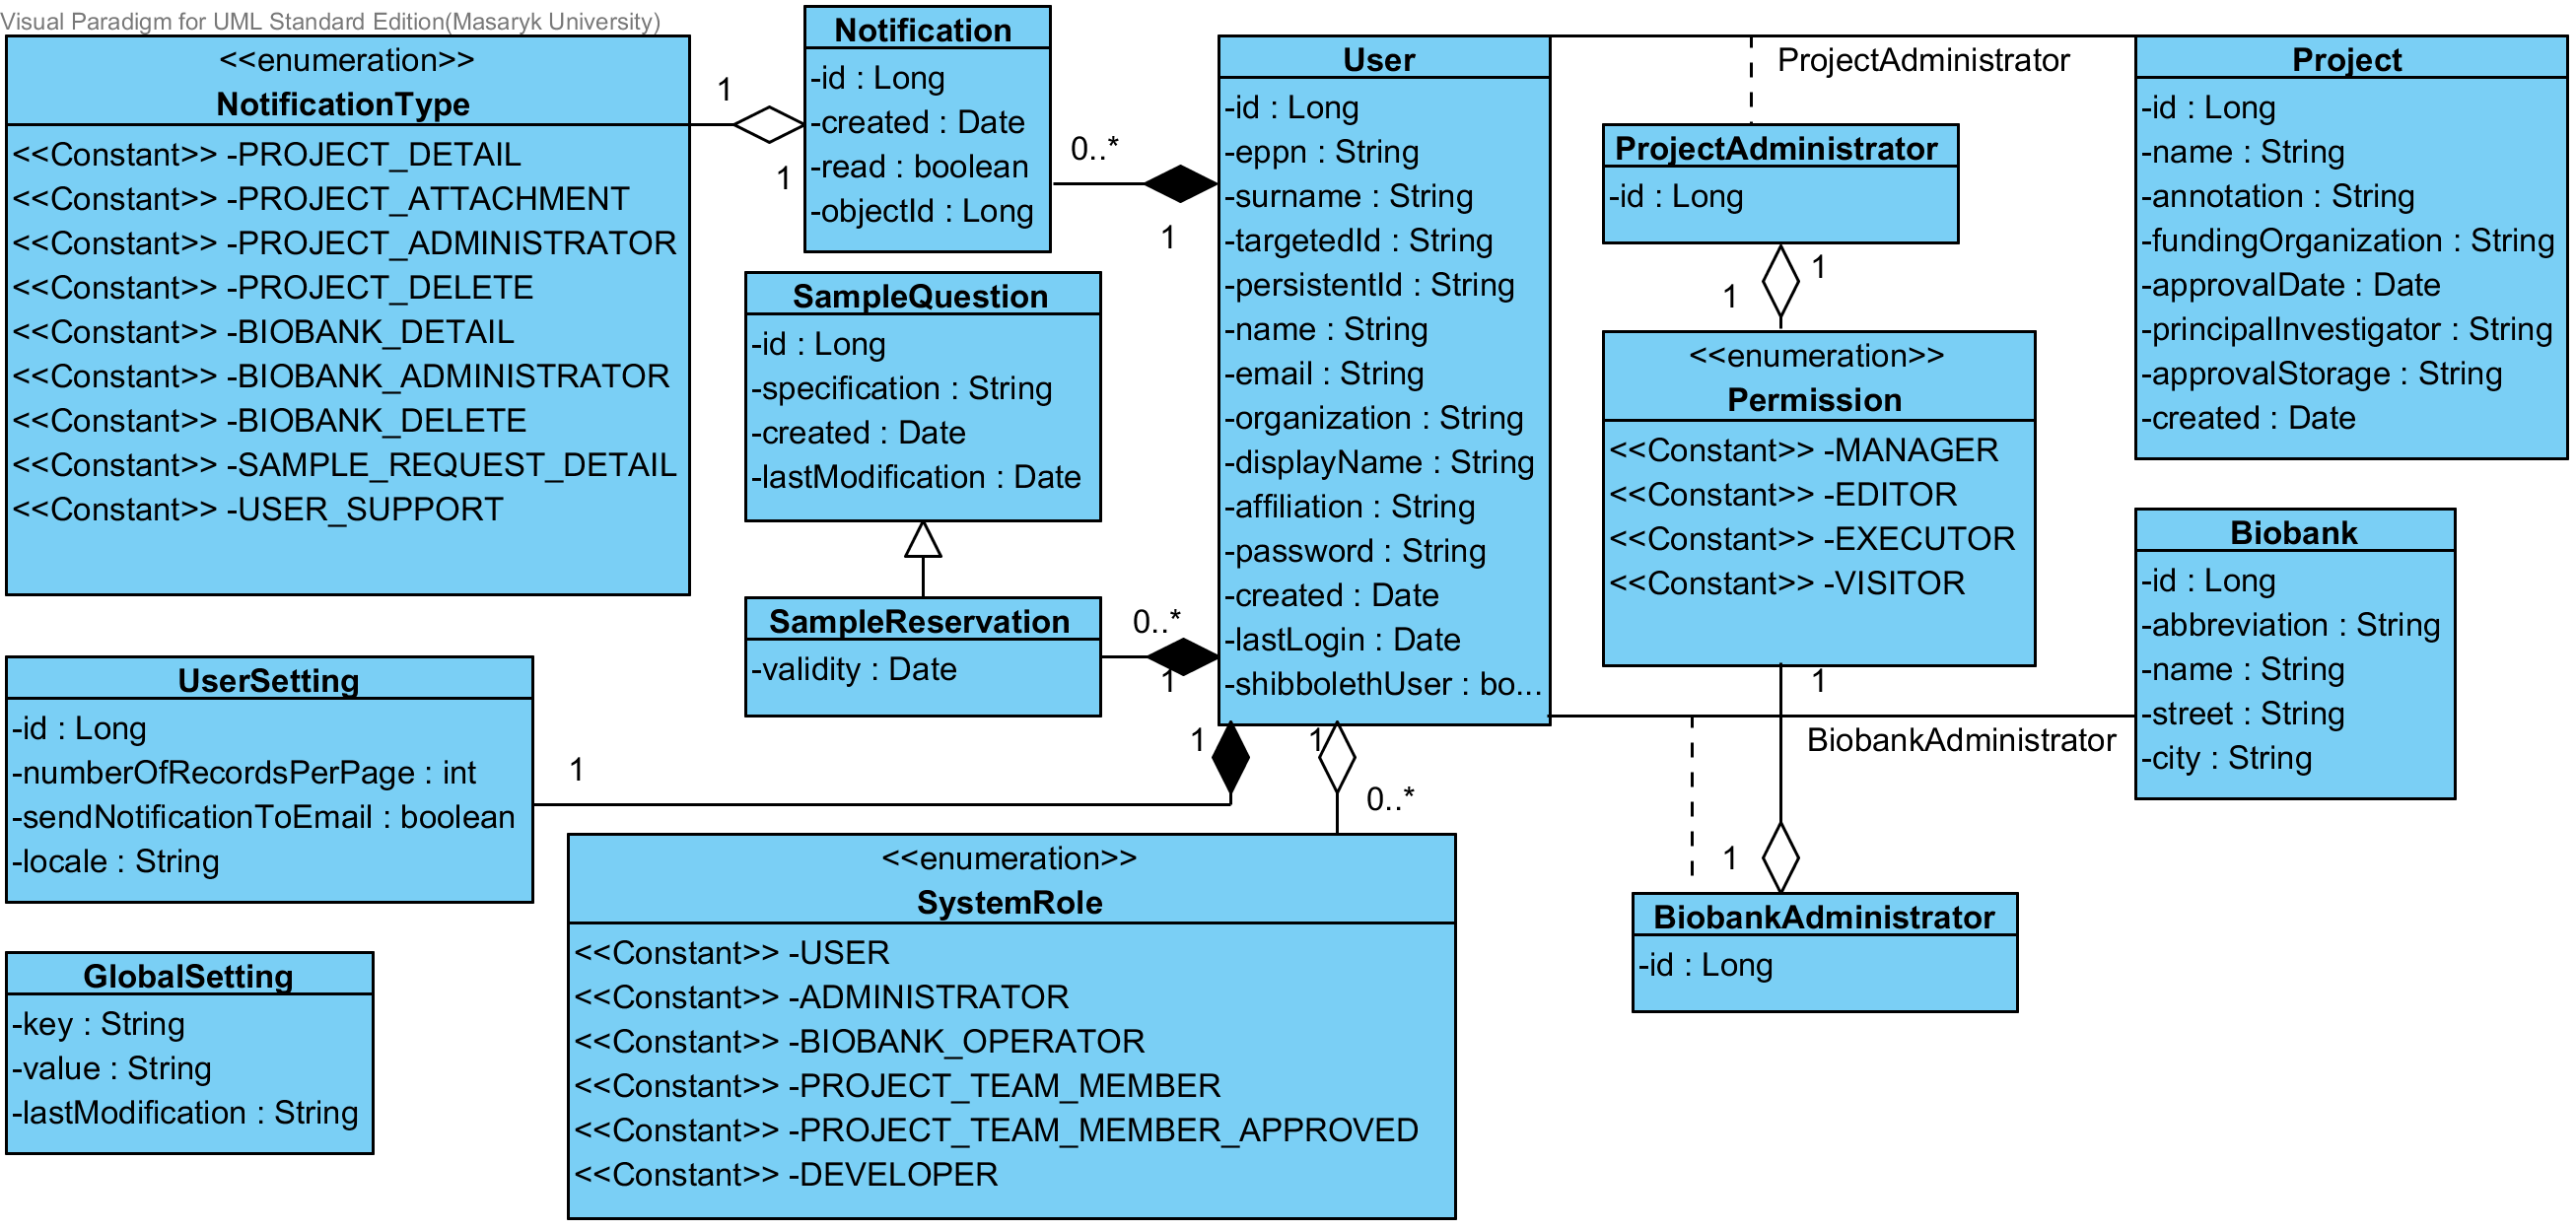
\includegraphics[width=\textwidth]{UserView}
\caption{UML class diagram tříd souvisejících s~třídou \textit{User}}
\label{fig:index:uml:class:user}
\end{center}
\end{figure}

% ------------------------------------------------------------------------   
% ------------------------------------------------------------------------   
\section{Projekt}
Objekt \textit{Project} představuje záznam o~existujícím podaném projektu. Většina ukládaných atributů vychází z~formálních náležitostí souvisejících s~existujícím projektovým záměrem:
\begin{compactitem}
	\item name -- název projektu,
	\item fundingOrganization -- kdo projekt financuje,	
	\item approvedBy -- kým byl projekt schválen. Schvalováním je v~tomto kontextu myšlen proces mimo aplikaci - tj. nikoli formální kontrola administrátory \ProjectName
	\item approvalStorage -- kde je fyzický souhlas uložen,
	\item principalInvestigator -- hlavní řešitel projektu. Položka je ukládána jako obyčejné textové pole pro případ, že by dotyčná osoba nebyla autorizovaná k~přístupu do systému (např. zaměstnanec instituce nezačleněné do eduId).
	\item homeInstitution -- instituce, která projekt zaštiťuje,
	\item approvalDate -- datum schválení projektového záměru,
	\item annotation -- textový popis projektového záměru.
\end{compactitem}
Všechny jmenované atributy kromě anotace jsou považované za konstantní v~průběhu životního cyklu projektu. Ostatní atributy souvisí s~aplikační logikou. 

\begin{figure}[h!]
\begin{center}
	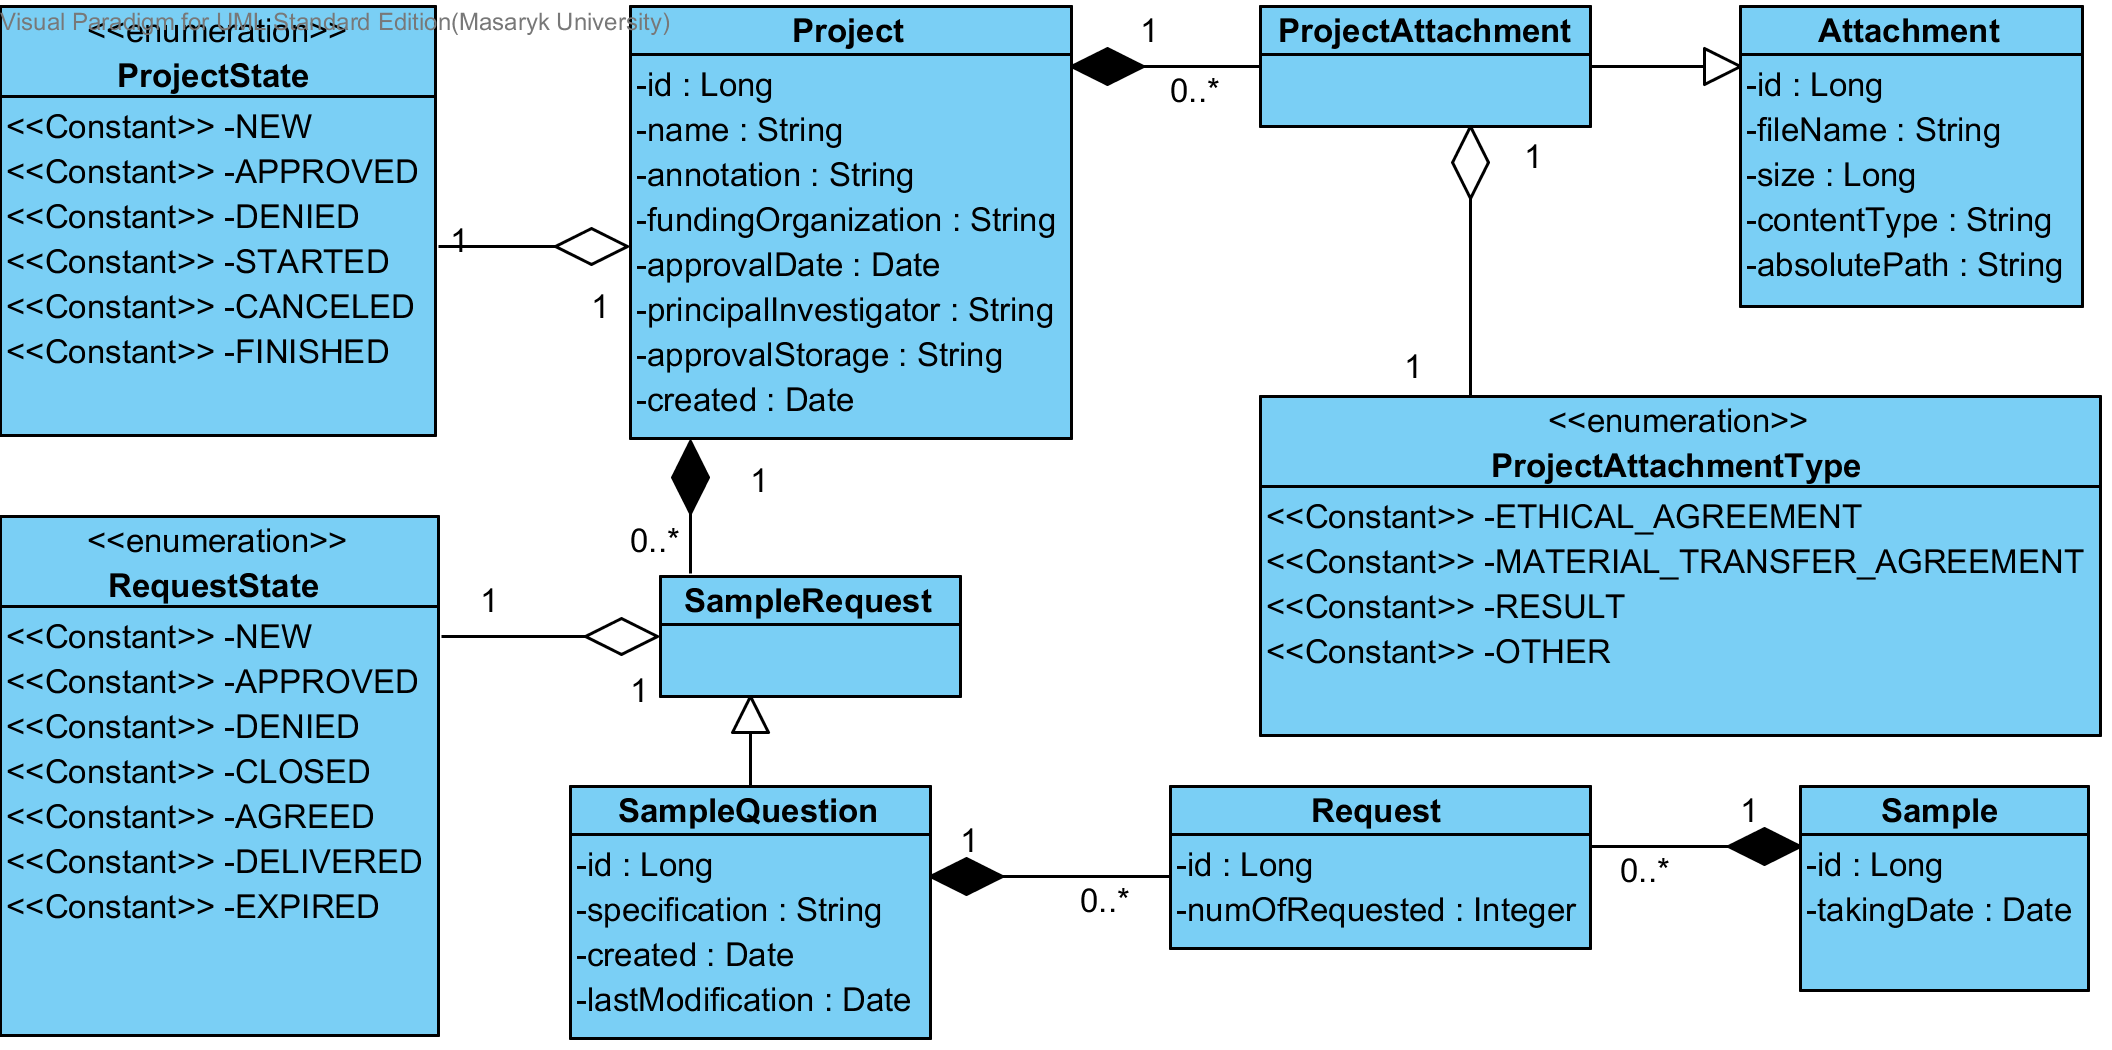
\includegraphics[width=\textwidth]{ProjectView}
\caption{UML class diagram tříd souvisejících s~projektem}
\label{fig:index:uml:class:project}
\end{center}
\end{figure}

% ------------------------------------------------------------------------   
\subsection{Příloha}
Při nahrání projektu je nutné nahrát podepsaný formulář MTA. Model aplikace umožňuje, aby bylo nahráno libovolné množství příloh k~projektu. Pro každou přílohu je možné definovat, jaký je její význam v~rámci projektu pro usnadnění orientace mezi soubory. U~kategorizace příloh se nepočítá s~velkými změnami, takže byl pro jejich definování použit výčtový typ.

% ------------------------------------------------------------------------   
\subsection{Životní cyklus projektu}
Po založení je projekt označen jako \textit{nový}. Po kontrole formálních náležitostí administrátorem může být \textit{schválen} nebo \textit{zamítnut}. V~kontextu schváleného projektu je již možné žádat o~vzorky. Projekt s~alespoň jednou žádostí je považován za \textit{zahájený}. Na konci realizace lze označit projekt za \textit{dokončený}. \textit{Dokončený} projekt v~systému i~nadále zůstává pro archivaci, ale je již pouze pro čtení a~nelze v~jeho kontextu žádat o~vzorky. 
V~aplikaci je definována i~možnost zrušit schválený projekt (v~diagramu značeno přerušovanou čarou). Tato funkce ale není ve stávající verzi zpřístupněna na uživatelském webovém rozhraní. Životní cyklus projektu je znázorněn na diagramu~\ref{fig:implementace:projekt:cyklus}. Barevně jsou znázorněny události iniciované {\color{palatinatepurple}administrátory} a~{\color{cyan}členem projektového týmu}. 

\begin{figure}[hbtp]
\begin{center}
\begin{tikzpicture}[->,>=stealth',shorten >=1pt,auto,node distance=45mm,
  thick,main node/.style={ellipse,draw}]

  \node[main node] (novy) {Nový};
  \node[main node] (schvaleny) [right of=novy] {Schválený};
  \node[main node] (zamitnuty) [below = 20mm of schvaleny] {Zamítnutý};
  \node[main node] (zapocaty) [right of=schvaleny] {Započatý};
  \node[main node,  dashed] (zruseny) [above = 20mm of zapocaty] {Zrušený};
  \node[main node] (dokonceny) [below = 20mm of zapocaty] {Dokončený};

  \path[every node/.style={font=\sffamily\small}]
    (novy) 
        edge [right, palatinatepurple] node[sloped, above] {Schválit} (schvaleny)
        edge [right, palatinatepurple] node[sloped, above] {Zamítnout} (zamitnuty)
    (schvaleny)
				edge [right, cyan] node[sloped, above] {Žádost} (zapocaty)
        edge [right, cyan] node[sloped, above] {Dokončit} (dokonceny)
        edge [right, dashed, palatinatepurple] node[sloped, above] {Zrušit} (zruseny)
    (zamitnuty)
	  (zapocaty)
				edge [right, cyan] node[right] {Dokončit} (dokonceny)
        edge [right, dashed, palatinatepurple] node[right] {Zrušit} (zruseny)
    (zruseny)
    (dokonceny);

\end{tikzpicture}
\caption{Životní cyklus projektu}
\label{fig:implementace:projekt:cyklus}
\end{center}
\end{figure}

% ------------------------------------------------------------------------   
\subsection{Životní cyklus žádosti a~rezervace vzorků}
Uživatel s~projektovým záměrem, ale bez splněných formálních náležitostí, může podat žádost o~rezervaci vzorků. Ta je \textit{schválena} v~situaci, kdy banka má kapacitu na to, aby žádosti vyhověla (tj. mají dostatek vzorků). V~opačném případě je rezervace \textit{zamítnuta}. Ke schválené rezervaci je možné přiřadit konkrétní počty alikvoty vzorků. Když je seznam vzorků kompletní, je žádost \textit{uzavřena}. Od chvíle uzavření běží lhůta platnosti rezervace. Když tato lhůta vyprší, je žádost označena jako \textit{expirovaná} a~alokované vzorky jsou uvolněny.
Žádost lze přiřadit k~vybranému, schválenému projektu, ke kterému má uživatel oprávnění spravovat žádosti i~vzorky. Tím je možné se vyhnout propadnutí rezervace. 
Na základě pouhé rezervace není možné fyzické vzorky získat. Životní cyklus rezervace je znázorněn v~diagramu~\ref{fig:implementace:rezervace:cyklus}, zatímco cyklus žádosti je v~diagramu~\ref{fig:implementace:zadost:cyklus}. Pro oba diagramy platí barevné odlišení iniciátorů znázorněných událostí: {\color{palatinatepurple}administrátor biobanky}, {\color{cyan}uživatel}/{\color{cyan}člen projektového týmu}. 

\begin{figure}[hbtp]
\begin{center}
\begin{tikzpicture}[->,>=stealth',shorten >=1pt,auto,node distance=45mm,
  thick,main node/.style={ellipse,draw}]

  \node[main node] (novy) {Nová};
  \node[main node] (schvalen) [right of=novy] {Schválena};
  \node[main node] (zamitnut) [below = 20mm of schvalen] {Zamítnuta};
  \node[main node] (uzavren) [right of=schvalen] {Uzavřena};
  \node[main node] (expirovan) [above = 20mm of uzavren] {Expirovala};
	\node[main node] (zadost) [below = 20mm of uzavren] {Vytvořena žádost};
    
  \path[every node/.style={font=\sffamily\small}]
    (novy)
    	edge [right, palatinatepurple] node[sloped, above] {Schválit} (schvalen)
      edge [right, palatinatepurple] node[sloped, above] {Zamítnout} (zamitnut)
    (schvalen)
    	edge [right, palatinatepurple] node[sloped, above] {Zkompletovat} (uzavren)
    (zamitnut)
    (uzavren)
      edge [right] node[right] {Expirace} (expirovan)
			edge [right] node[right, cyan] {Přiřadit projektu} (zadost);
\end{tikzpicture}
\caption{Životní cyklus rezervace}
\label{fig:implementace:rezervace:cyklus}
\end{center}
\end{figure}

Počátek životního cyklu žádosti o~vzorky je totožný s~rezervací. V~situaci, kdy je žádost uzavřena pracovníkem biobanky, je umožněno aby žadatel sadu potvrdil nebo ji vrátil zpět k~doplnění. Tato volba se uplatní v~situaci, kdy vzorky nesplňují kladené požadavky. Žádost se tím vrátí do stavu \textit{schválena}, aby bylo opět možné editovat sadu vzorků.
Může také nastat situace, že o~stejné vzorky bylo požádáno ve více biobankách a~více žádostí bylo vyřízeno kladně, takže je pro projekt alokováno více zdrojů, než je nutné. V~této situaci může správce projektu žádost smazat a~tím alokované vzorky uvolnit.
Po schválení vybrané sady žadateli jsou tyto vzorky fyzicky připraveny k~odebrání. Žádost s~fyzicky předanými vzorky je označena jako \textit{doručena}.

\begin{figure}[hbtp]
\begin{center}
\begin{tikzpicture}[->,>=stealth',shorten >=1pt,auto,node distance=45mm,
  thick,main node/.style={ellipse,draw}]

  \node[main node] (novy) {Nová};
  \node[main node] (schvalen) [right of=novy] {Schválena};
  \node[main node] (zamitnut) [below = 20mm of schvalen] {Zamítnuta};
  \node[main node] (uzavren) [right of = schvalen] {Uzavřena};
  \node[main node] (potvrzen) [below = 20mm of uzavren] {Potvrzena};
  \node[main node] (vydan) [below = 20mm of potvrzen] {Vybavena};
    
  \path[every node/.style={font=\sffamily\small}]
    (novy)
    	edge [right, palatinatepurple] node[sloped, above] {Schválit} (schvalen)
        edge [right, palatinatepurple] node[sloped, above] {Zamítnout} (zamitnut)
    (schvalen)
    	edge [right, palatinatepurple] node[sloped, above] {Zkompletovat} (uzavren)
    (zamitnut)
    	
    (uzavren)
    	edge [right, cyan] node[right] {Vyhovuje} (potvrzen)
        edge [bend left, cyan] node[sloped, above] {Nevyhovuje} (schvalen)
    (potvrzen) 
    	edge [right, palatinatepurple] node[right] {Předat} (vydan)
    ;

\end{tikzpicture}
\caption{Životní cyklus žádosti}
\label{fig:implementace:zadost:cyklus}
\end{center}
\end{figure}

% ------------------------------------------------------------------------   
% ------------------------------------------------------------------------   
\section{Biobanka}
Entita reprezentující instituci, zapojenou do projektu \ProjectName, která poskytuje biologický materiál ostatním. Atribut \textit{abbreviation} slouží pro kontrolu při parsování importů, že zpracovávaný XML soubor skutečně patří ke správné biobance a~nedošlo k~chybě při kopírování (např. spletení cílové cesty).

\begin{figure}[h!]
\begin{center}
	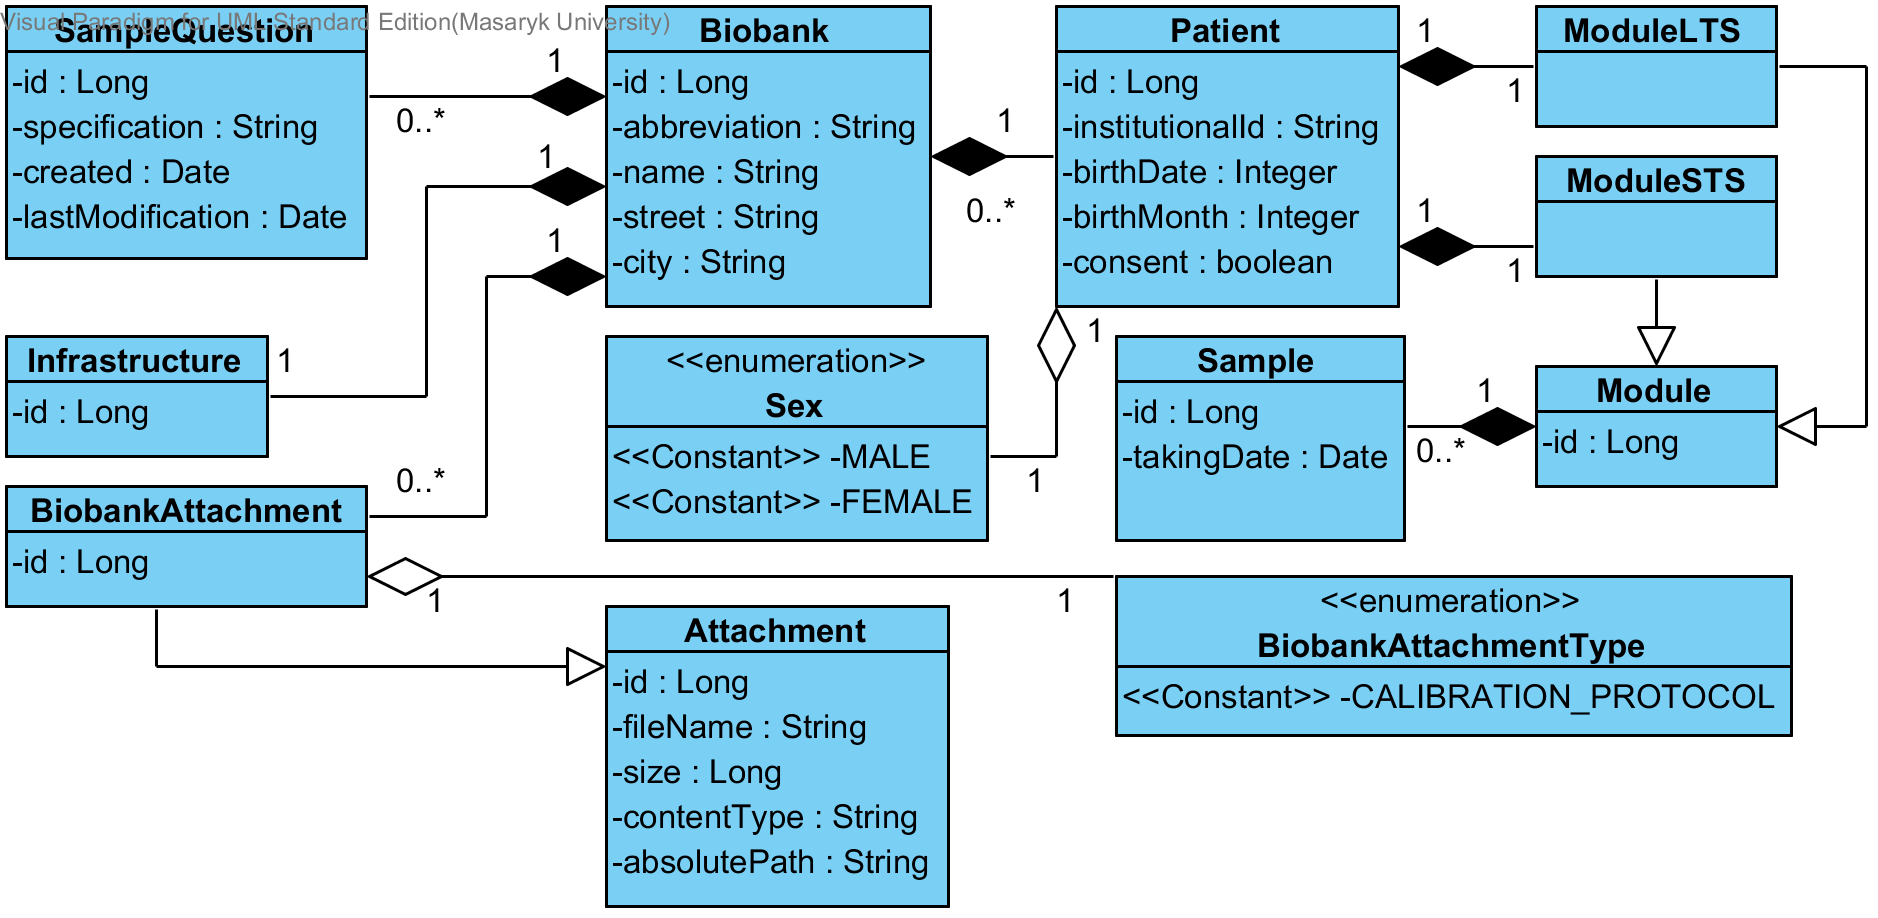
\includegraphics[width=\textwidth]{BiobankView}
\caption{UML class diagram tříd souvisejících s~biobankou}
\label{fig:index:uml:class:biobank}
\end{center}
\end{figure}

% ------------------------------------------------------------------------   
\subsection{Infrastruktura biobanky}
Diagram~\ref{fig:index:uml:class:infrastructure} popisuje, jakým způsobem je v~aplikaci uložena struktura repozitáře biobanky. Struktura vychází z~analýzy popsané v~kapitole~\ref{chapter:analysis:subsection:monitoring}.

\begin{figure}[h!]
\begin{center}
	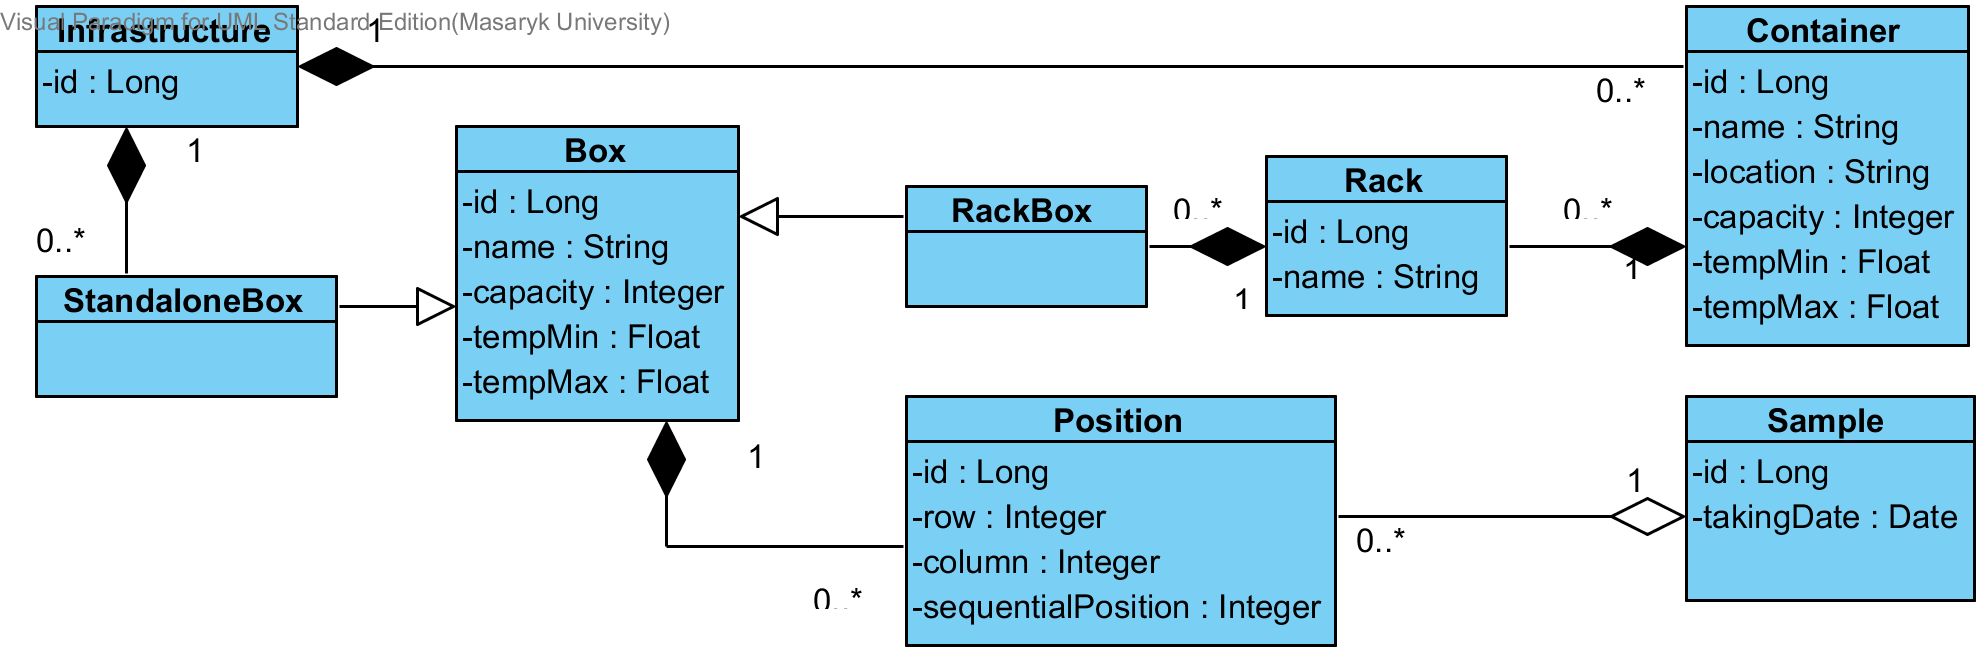
\includegraphics[width=\textwidth]{InfrastructureView}
\caption{UML class diagram popisující infrastrukturu biobanky}
\label{fig:index:uml:class:infrastructure}
\end{center}
\end{figure}

% ------------------------------------------------------------------------   
\subsection{Monitoring biobanky}
Kontejner může mít přiřazeno $0-n$ měření. Každé měření definuje pomocí enumeračního typu konkrétní měřenou fyzikální veličinu a~použité jednotky. Touto strukturou lze tedy modelovat různé počty teplotních i~jiných čidel, přiřazených ke kontejneru. 
Doba ponechání změřených dat v~databázi bude stanovena až na základě praktických zkušeností s~využíváním systému (faktické množství generovaných dat proti požadavkům na zpětné doložení nakládání s~daty).

\begin{figure}[h!]
\begin{center}
	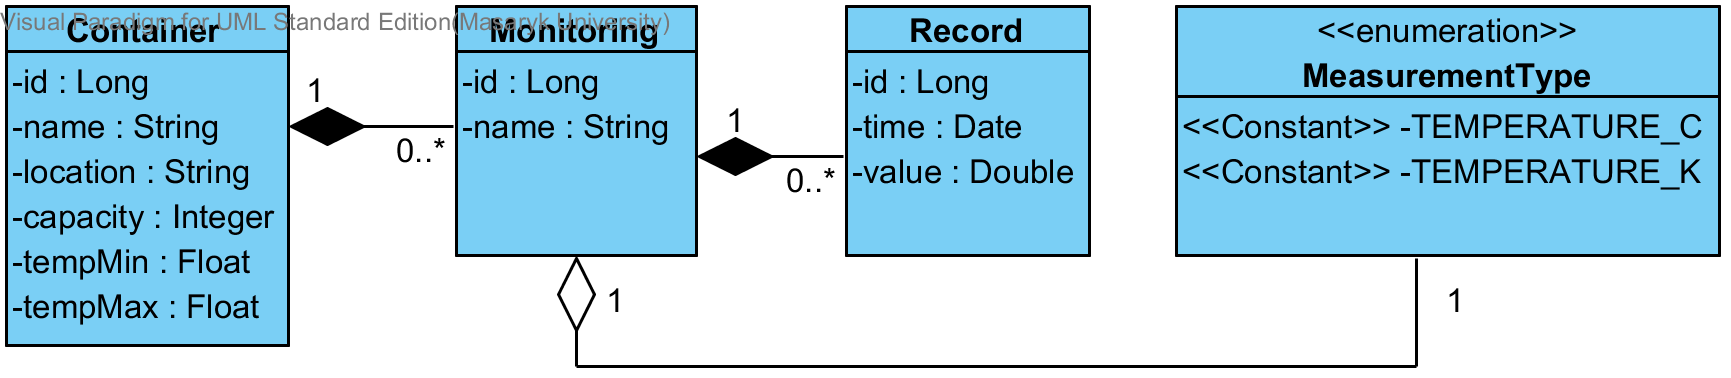
\includegraphics[width=\textwidth]{MonitoringView}
\caption{UML class diagram popisující sledování fyzikálních parametrů v~prvcích infrastruktury}
\label{fig:index:uml:class:monitoring}
\end{center}
\end{figure}


% ------------------------------------------------------------------------   
\subsection{Kalibrační protokoly}
Pro ověření, že data z~monitoringu biobanky jsou relevantní k~posouzení kvality uložení, je třeba minimálně jednou za dva roky měřící přístroje zkalibrovat. Protokoly o~kalibraci je možné uložit jako dokumenty vztahující se k~biobance.


% ------------------------------------------------------------------------   
% ------------------------------------------------------------------------   
\section{Popis uložených vzorků}
Objektový návrh~\ref{fig:index:uml:class:sample} vychází ze struktury exportů popsaných v~předchozí kapitole.

\begin{figure}[h!]
\begin{center}
	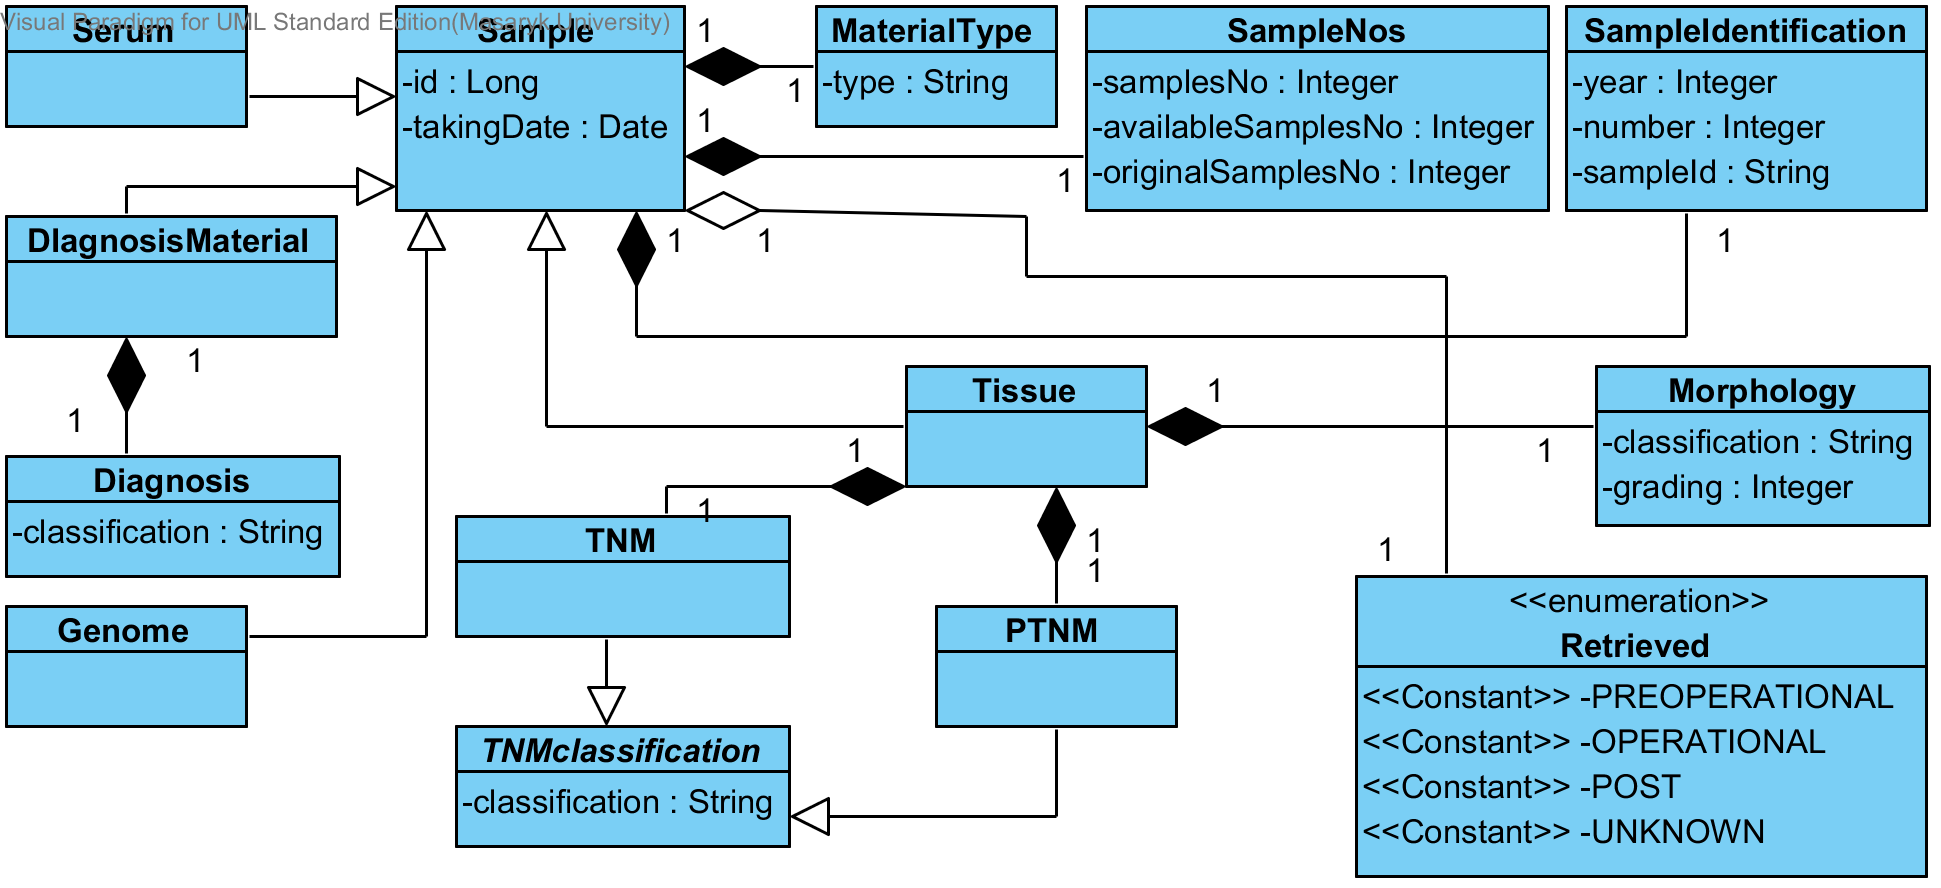
\includegraphics[width=\textwidth]{SampleView}
\caption{UML class diagram popisující biologický materiál}
\label{fig:index:uml:class:sample}
\end{center}
\end{figure}


% ------------------------------------------------------------------------   
% ------------------------------------------------------------------------   
\section{Autorizace uživatelů}
Pro stanovení, které zdroje systému může uživatel používat byly stanoveny systémové role. Pro jemnější členění oprávnění vztažených ke konkrétnímu objektu byly definovány úrovně oprávnění.

% ------------------------------------------------------------------------   
\subsection{Systémové role}
Systémové role jsou definovány enumerační třídou \textit{SystemRole} z~package \textit{cz.bbmri.entities.enumeration}. 

\paragraphNewLine{Uživatel}
Uživatel je implicitní role každého uživatele oprávněného přistupovat k~indexu. Při autentizaci uživatele je na základě parametrů získaných z~eduId stanoveno, zda může být dotyčnému uživateli umožněno vstoupit do systému - každý kdo je vpuštěn má roli \textit{uživatel}. Pohyb uživatele bez role \textit{uživatel} je považován za chybu.
Uživateli s~touto rolí je dovoleno:
\begin{compactitem}
	\item přistupovat ke svým vlastním údajům a~k~osobnímu nastavení
	\item podávat rezervace na vzorky
	\item nahrávat informace o~projektech
	\item zobrazit kontakty na vývojáře a~administrátory systému
	\item zobrazit všechny biobanky registrované v~systému.
\end{compactitem}

\paragraphNewLine{Správce biobanky}
Uživateli s~oprávněním alespoň k~jedné biobance je přidělena systémová role \textit{správce biobanky}. Role samotná upravuje pouze položky v~menu. Autorizace pro provádění konkrétních operací je stanovena na základě oprávnění ke konkrétní instanci biobanky. 

\paragraphNewLine{Člen projektového týmu} 
Každý uživatel s~oprávněním alespoň k~jednomu projektu má systémovou roli \textit{člen projektového týmu}. Autorizace pro provádění konkrétních operací je stanovena na základě oprávnění ke konkrétní instanci projektu. 

\paragraphNewLine{Člen projektového týmu se schváleným projektem}
Systémovou roli \textit{člena projektového týmu se schváleným projektem} má každý uživatel s~oprávněním alespoň k~jednomu schválenému projektu. Při schválení některého z~projektů uživatele je role \textit{člen projektového týmu} nahrazena za \textit{člen projektového týmu se schváleným projektem}. Naopak je role odebrána při smazání nebo dokončení schváleného projektu.
Uživateli s~touto rolí je dovoleno:
\begin{compactitem}
	\item zobrazit monitoring teploty ve všech biobankách.
\end{compactitem}

\paragraphNewLine{Vývojář}
Systémová role \textit{vývojář} je určena pro uživatele systému, kteří se podílí na jeho vývoji.
Uživateli s~touto rolí je dovoleno:
\begin{compactitem}
	\item založit biobanku, smazat biobanku
	\item zobrazit veškeré informace zobrazované na webu bez možnosti editace
	\item přiřadit nebo odebrat uživateli roli vývojáře nebo administrátora.
\end{compactitem}

\paragraphNewLine{Administrátor}
Systémová role \textit{administrátor} přísluší koordinátorům projektu \ProjectName.
Uživateli s~touto rolí je dovoleno:
\begin{compactitem}
	\item založit biobanku, smazat biobanku
	\item zobrazit veškeré informace zobrazované na webu bez možnosti editace
	\item přístup ke globálnímu nastavení systému
	\item přiřadit nebo odebrat uživateli roli vývojáře nebo administrátora.
\end{compactitem}

% ------------------------------------------------------------------------   
\subsection{Oprávnění k~projektu}
V~průběhu realizace se ukázalo, že je žádoucí, aby kardinalita mezi projektem a~uživatelem nebyla $n:1$, ale $n:m$. Oprávnění k~úpravě projektu ale nemůže být vázané na systémovou roli, protože pak by při špatném rozvržení .jsp stránek hrozilo, že bude umožněna manipulace s~cizím projektem. Z~hlediska spolupráce více lidí na projektu je také vhodné umožnit delegování odpovědnosti. Tyto jmenované argumenty vedly k~potřebě rozlišovat úroveň oprávnění přístupu zvlášť ke každému projektu.
Mezi jednotlivými oprávněními je vztah inkluze, tj. vyšší zahrnuje vše z~nižšího. Oprávnění jsou definována v~třídě cz.bbmri.entities.enumeration.Permission.

\paragraphNewLine{Návštěvník (Visitor)} 
Uživateli s~oprávněním \textit{návštěvník} je umožněno zobrazit všechny stránky související s~projektem, ke kterému se oprávnění pojí - tj. detail projektu, projektový tým, přílohy a~další. Není mu ale umožněno data jakkoli měnit. Uživatel nenese žádnou odpovědnost za aktivitu v~systému.

\paragraphNewLine{Výkonný pracovník (Executor)} 
Oprávnění \textit{executor} umožňuje uživateli vykonávat následující operace:
\begin{compactitem}
	\item označit projekt jako dokončený
	\item pracovat s~žádostmi o~vzorky (vytvoření, schvalování,\ldots)
	\item manipulace s~přílohami projektu
\end{compactitem}

\paragraphNewLine{Pracovník s~možností editace (Editor)}
Uživateli s~oprávněním \textit{editor} je umožněno měnit editovatelné položky související s~projektem.

\paragraphNewLine{Manager}
Nejvyšší oprávnění umožňující manipulovat se složením týmu a~s~oprávněními jednotlivých osob.

% ------------------------------------------------------------------------   
\subsection{Oprávnění k~biobance}
Stejná motivace jako u~projektu vedla k~zavedení úrovní oprávnění i~pro biobanky. Oprávnění jsou definována následovně. 

\paragraphNewLine{Návštěvník (Visitor)} 
Obdobně jako u~projektu, je i~u~biobanky oprávnění visitor omezeno výhradně na zobrazení dat bez možnosti jejich úpravy. 

\paragraphNewLine{Výkonný pracovník (Executor)}
Uživatel s~oprávněním \textit{executor} může v~kontextu biobanky vykovánavat následující operace:
\begin{compactitem}
	\item schvalovat projekty
	\item manipulace s~žádostmi o~vzorky
\end{compactitem}

\paragraphNewLine{Pracovník s~možností editace (Editor)} 
Uživateli s~oprávněním \textit{editor} je umožněno měnit editovatelné položky související s~biobankou.
\begin{compactitem}
	\item manuální vytváření infrastruktury biobanky (kontejnery, stojany, ...)
	\item manuální vytváření pacientů a~vzorků
	\item možnost měnit editovatelné položky biobanky
\end{compactitem}

\paragraphNewLine{Manager}
Nejvyšší oprávnění umožňující manipulovat se složením týmu a~s~oprávněním jednotlivých osob.











% ------------------------------------------------------------------------   
% ------------------------------------------------------------------------      
% Implementace
% ------------------------------------------------------------------------   
\chapter{Implementace}\label{chapter:implementation}
Aplikace je provozována na serveru Metacentra\footnote{\url{http://www.metacentrum.cz/}}, na adrese \textit{cloud19.cerit-sc.cz}. Druhý alokovaný server, přístupný na adrese \textit{cloud20.cerit-sc.cz}, slouží pro testovací účely. V~obou případech se jedná o~linuxové stroje s~operačním systémem \textit{Debian Squeeze} verze $6.0$. Stroje jsou vybaveny procesory Intel Xeon E312xx Sandy Bridge a~disponují 6GB operační paměti.
Pro nasazení aplikace byly zaregistrovány domény \url{www.bbmri.cz} a~\url{index.bbmri.cz}, které odkazují na produkční server \url{cloud19.cerit-sc.cz}. Domény jsou ve správě informatického oddělení MOÚ.
Dle požadavků bylo nutné zajistit šifrování komunikace se serverem. Proto byl pro uvedené domény vystaven certifikát, používaný pro HTTPS. 
Doména \url{www.bbmri.cz} má čistě informativní charakter, zatímco doména \url{https://index.bbmri.cz} vede do vlastní aplikace.
Pro vývoj aplikace byl používán repozitář github\footnote{Adresa repozitáře: \url{https://github.com/Ondrej-vojtisek/bbmri}}. 
Cílem následující kapitoly je vysvělit argumenty pro volbu použitých technologií a~vysvětlit některé nestandardní implementační detaily.


% ------------------------------------------------------------------------   
% ------------------------------------------------------------------------    
\section{Použité technologie}
Aplikace je implementována v~Javě verze 7, nicméně nevyužívá žádných syntaktických \uv{novinek} Javy 7 a~kód je bez úprav kompilovatelný a~spustitelný i~v~Javě verze 6. 

% ------------------------------------------------------------------------   
\subsection{Maven}
Pro sestavení aplikace byl používán nástroj Maven\footnote{\url{http://maven.apache.org/}}. Programátor v~souboru pom.xml nadefinuje, které knihovny a~programovací nástroje aplikace používá, včetně specifikace verze těchto nástrojů. Maven tyto závislosti stáhne a~aplikaci sestaví. Pro vývoj představuje použití Mavenu usnadnění, protože vývojář nemusí řešit tranzitivní závislosti jednotlivých knihoven a~má lepší přehled nad verzemi použitých knihoven. 

% ------------------------------------------------------------------------   
\subsection{Hibernate}
Pro ukládání dat a~pro přístup k~nim byl použit ORM (Object-Relational Mapping\footnote{Způsob konverze dat mezi relační databází a~objektem objektově orientovaného jazyka.}) JPA (Java Persistence API). JPA je rozhraní (API), které definuje, jakým způsobem jsou objekty mapovány na tabulky relační databáze. Vazby mezi entitami aplikace jsou definovány pomocí anotací ve zdrojovém kódu. Parametry připojení k~databázi jsou JPA poskytnuty konfiguračními soubory viz~\ref{chapter:implementation:section:konfiguration}. JPA není závislé na konkrétní implementaci databáze.
Hibernate je implementace JPA, která byla v~aplikaci použita. Konkrétně byla použita verze 3.6.10. Alternativou k~Hibernate je např. OpenJPA\footnote{\url{https://openjpa.apache.org/}}. Argumentem pro volbu Hibernate byl explicitní požadavek v~zadání práce, stanovený s~cílem sjednotit používané technologie v~projektech realizovaných na ÚVT MUNI (resp. v~centru CERIT-SC). 
Hibernate za vývojáře zajišťuje vytvoření databáze podle datového modelu (popsaného anotacemi entit aplikace). Databáze je vytvářena automaticky. Hibernate zvládne i~průběžně měnit strukturu databáze podle aktuálních změn anotací. Vývojář musí mít pouze na paměti, že po úpravách mohou v~databázi zůstat nekonzistentní objekty.
Pro dotazování nad databází se používá JPQL (Java Persistence Query Language) namísto běžného SQL používaného v~relačních databázích. JPQL umožňuje pokládat dotazy na základě znalosti entit a~do bez znalosti jejich skutečného uložení v~databázi (např. kladení dotazů bez znalosti pojmenování tabulek).

% ------------------------------------------------------------------------   
\subsection{Spring}
Jako základ pro implementaci aplikační vrstvy aplikace byl použit aplikační rámec Spring\footnote{\url{http://spring.io/}}, který umožňuje automatické dynamické vytváření potřebných objektů za běhu aplikace. Tento mechanismus se nazývá \textit{dependency injection} a~pro programátora představuje usnadnění, neboť programátor nemusí dohlížet na incializaci kontrolovaných objektů. Objekty, jejichž závislost má spravovat Spring, jsou v~kódu označeny anotací \textit{@Autowired}. Jedná se o~všechny třídy implementující rozhraní DAO a~Servisní (resp. aplikační) vrstvy.
Alternativou pro Spring je aplikační rámec EJB (Enterprise Java Beans).

% ------------------------------------------------------------------------   
\subsection{Stripes}
Stripes je MVC (Model-View-Controller) aplikační rámec pro prezentační vrstvu Java EE aplikací. Hlavní myšlenkou autorů frameworku byla snaha minimalizovat nutnou konfiguraci pomocí XML souborů a~umožnit konfiguraci pomocí anotací zavedených v~Javě 5. Stripes řeší vše nutné pro webovou vrstvu aplikace, jako validaci vstupů, lokalizaci obsahu, mechanismus informování uživatele zprávami, atd. Stripes mimo jiné obsahuje nástroje pro tvorbu šablon JSP stránek, které výrazně napomáhají snížit duplicitu kódu.
Využití frameworku bylo doporučeno na základě zvyklostí s~vývojem Java aplikací na ÚVT.

\paragraph*{Stripesstuff} -- Použitá sada rozšíření k~webovému rámci Stripes, usnadňující mimo jiné implementaci zabezpečení a~lokalizace webové aplikace. 

% ------------------------------------------------------------------------   
\subsection{Styl webu a~JavaScript}
Pro vizuální vzhled aplikace byl vybrán webový rámec bootstrap\footnote{\url{http://getbootstrap.com/}} ve verzi 2.3.2. Bootstrap je kolekce HTML kódu, CSS stylů a~u~dynamičtějších prvků webu (např. panel pro výběr data nebo výběr a~nahrání souboru z~disku) i~souvisejících jQuery knihoven. Společně tak vytváří pestrou sadu webových komponent s~jednotnou vizuální podobou, umožňující rychlé nasazení prototypu s~prezentovatelným designem. 

JQuery bylo použito kromě komponent Bootstrapu také pro zobrazení dat z~monitoringu fyzikálních parametrů biobank v~grafu. Pro tuto funkci byla použita knihovna Flot\footnote{\url{www.flotcharts.org}} 


% ------------------------------------------------------------------------   
% ------------------------------------------------------------------------   
\section{Práce s~daty}

% ------------------------------------------------------------------------   
\subsection{Organizace uložení dat}\label{chapter:implementation:subsection:organizationOfDataStorage}
Aplikace manipuluje s~množstvím různorodých dat, která se budou v~systému nacházet různě dlouhou dobu a~která do systému vstupují různými způsoby. Pro organizaci souborů aplikace slouží složka definovaná parametrem \textit{StoragePath} v~konfiguračním souboru \textit{my.properties} (výchozí hodnota je \textit{/home/bbmri\_data}). Tato složka slouží k~uložení veškerých dat souvisejících s~aplikací.

Projektové soubory (\textit{ProjectAttachment} v~UML diagramech) jsou uloženy uvnitř složky \textit{project\_files/id}, kde \textit{id} je identifikátor projektu. 

Soubory související s~biobankou jsou uloženy uvnitř složky \textit{biobank\_files} ve složce konkrétní biobanky (pojmenované podle identifikátoru). Adresář biobanky obsahuje složky: 
\begin{compactitem}
	\item \textit{patient\_data} -- pacientská data
	\item \textit{monitoring\_data} -- data popisující zaplnění biobanky
	\item \textit{temperature\_data} -- hodnoty z~měřidel z~biobanky
	\item \textit{calibration\_data} -- zaslané kalibrační protokoly
	\item \textit{patient\_data\_archive} -- archiv pacientských dat
	\item \textit{monitoring\_data\_archive} -- archiv zaplnění biobanky
	\item \textit{temperature\_data\_archive} -- archiv hodnot z~měřidel
\end{compactitem}

Ve výchozím nastavení je součástí složky \textit{/home/bbmri\_data} také soubor \textit{bbmri\_logger.log} obsahující logovací záznamy aplikace. 

% ------------------------------------------------------------------------   
\subsection{Import a~zpracování dat}\label{chapter:implementation:subsection:import}
Jak již bylo zmíněno výše, data budou do systému automatizovaně nahrávána formou XML importů. Data jsou podle zdroje nebo kontextu nahrávána do složky příslušné biobanky a~podle typu dat je zvolena konkrétní podsložka. Např. pacientská data z~MOÚ (za předpokladu, že PostgreSQL přidělí MOÚ unikátní identifikátor $= 1$) budou importována do složky \textit{/bbmri\_data/biobank\_files/1/patient\_data}. Data jsou sice anonymizovaná, ale i~tak je vysoce nežádoucí, aby se dostala mimo systém. Z~toho důvodu byly pro přenos uvažovány pouze metody využívající šifrování. Přenos dat zatím nebyl fakticky realizován, ale počítá se s~použitím protokolu SCP (Secure Copy) nebo SFTP (SSH File Transfor Protocol). 

Aplikace obsahuje v~balíku cz.bbmri.trigeredEvents třídy, jejichž metody nejsou spustitelné z~webového rozhraní, ale jsou spouštěny pouze automaticky. Automatické spouštění je implementováno pomocí anotace \textit{@Scheduled}\footnote{org.springframework.scheduling.annotation.Scheduled}, která umožňuje definovat, kdy má být metoda spuštěna plánovačem úloh \textit{cron}. 
Pro ilustraci následující anotace, spustí anotovanou metodu každý den deset minut po půlnoci. 
\begin{figure}[h!]
\centering
\begin{BVerbatim}
@Scheduled(cron = "10 0 * * * *")
\end{BVerbatim}
\end{figure}
Rutina pro import pacientů je nastavena, aby každý den minutu po půlnoci byly zkontrolovány adresáře všech biobank. Pokud adresář obsahuje nový soubor, tak je soubor přečten a~údaje jsou uloženy do databáze. Při úspěšném čtení dokumentu je XML soubor po vykonání rutiny přemístěn do složky \textit{patient\_data\_archive}, aby bylo možné zpětně pochopit chování systému a~zároveň nebyly opakovaně analyzovány stejné importy dat.
Obdobně jsou řešeny importy zaplnění i~naměřených dat, pouze s~rozdílem časů spuštění úloh.

Strukturu tříd, starajících se o~zpracování XML importů, popisuje UML diagram~\ref{fig:index:uml:class:parser}. Obě specializované třídy obsahují odkaz na konkrétní XML schéma (ve formátu XSD), takže jsou schopny provézt validaci dokument s~využitím metody abstraktní třídy. Dotazy na XML dokument jsou implementovány pomocí xPath.
Třída \textit{NamespaceContextMap} zajišťuje, aby byly xPath dotazované objekty chápány jako objekty popsané v~XML schématu.

Ve třídě \textit{MonitoringDataParser} je v~metodě \textit{getBoxPositions} použita třída \textit{PositionDTO} namísto \textit{Position} ukládané do databáze. Důvodem je, že parser nemá přístup do databáze a~tak nemůže získat instanci třídy \textit{Sample} v~databázi uloženou podle zjištěného identifikátoru. Snazší a~přehlednější, než vytvářet částečný objekt, jen s~identifikátorem instituce, je v~tomto případě předávat pouze načtený identifikátor. 

\begin{figure}[h!]
\begin{center}
	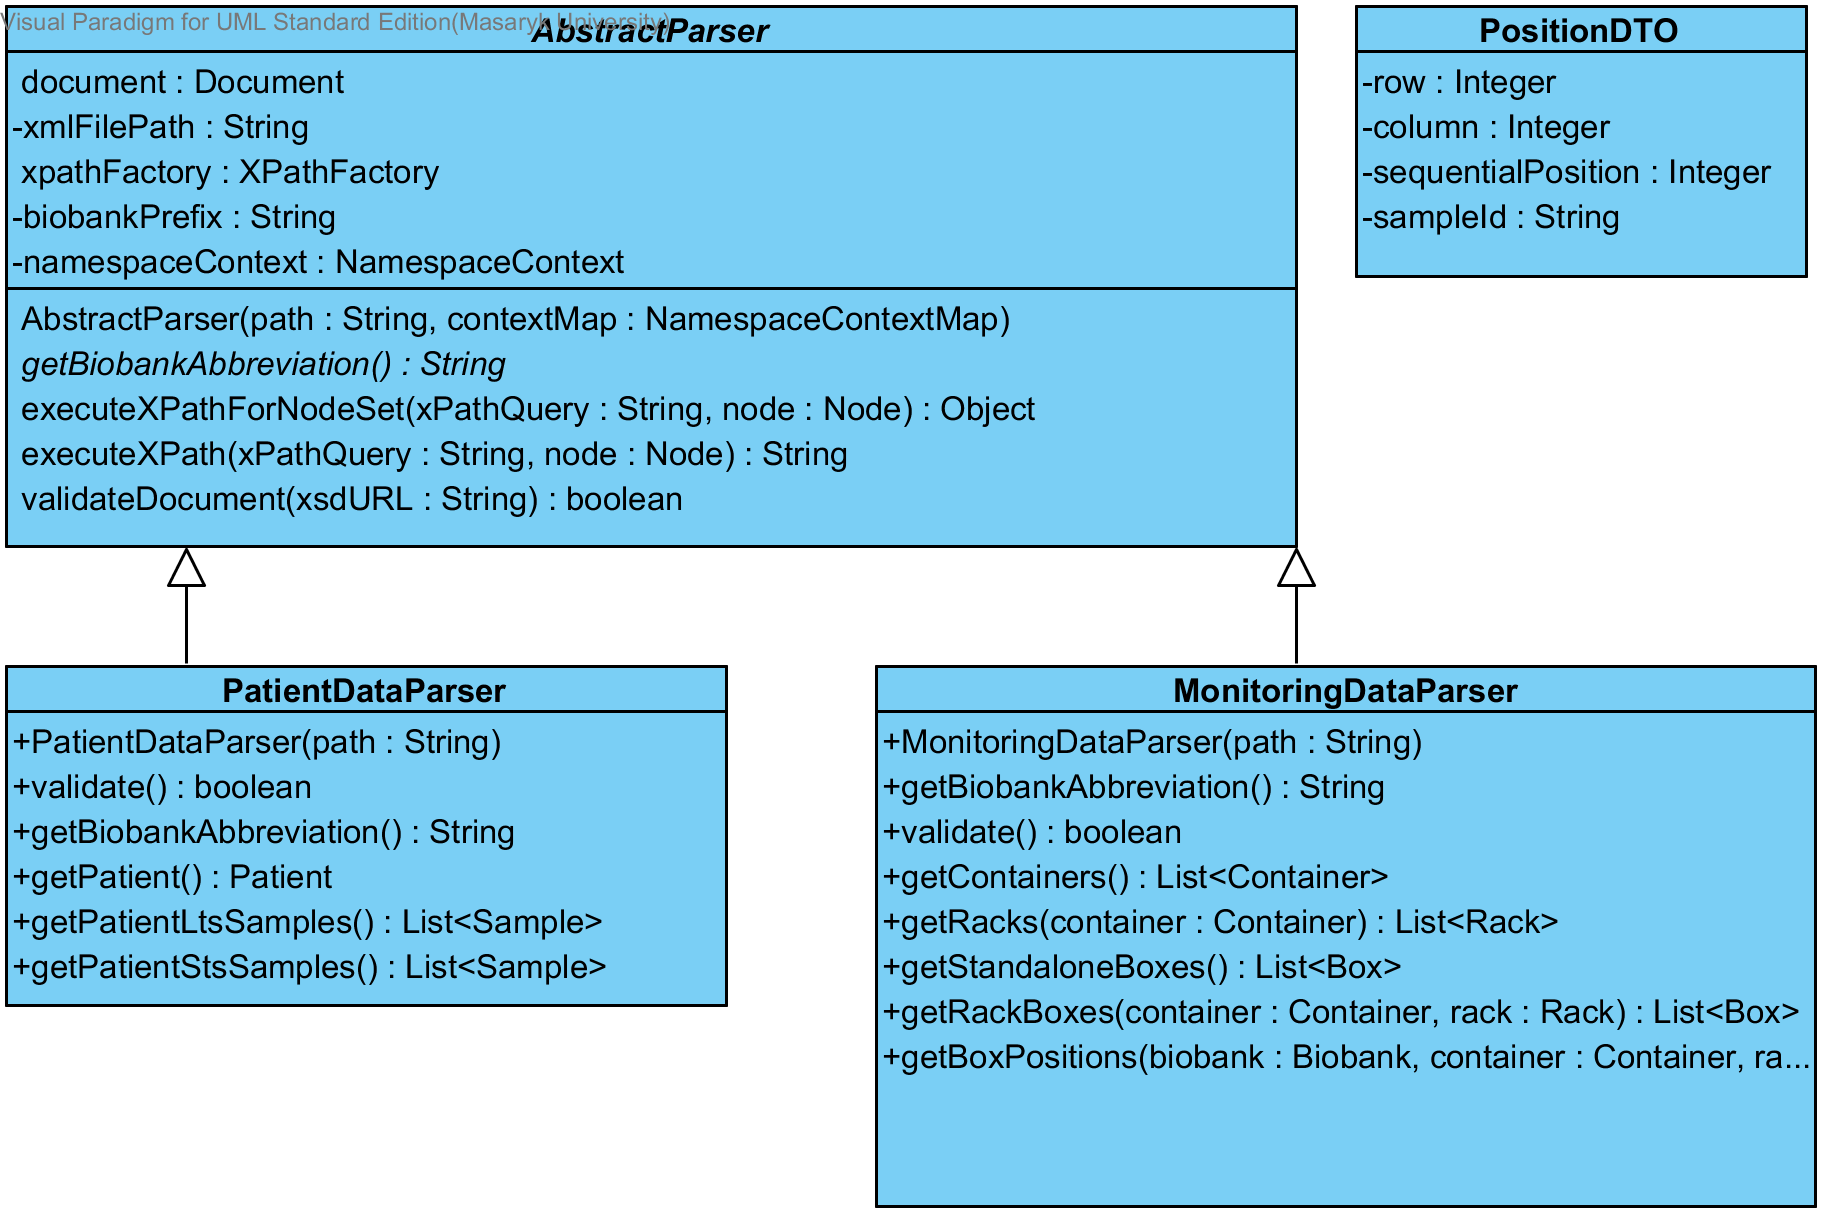
\includegraphics[width=\textwidth]{ParserView}
\caption{UML class diagram popisující třídy pro zpracování XML importů}
\label{fig:index:uml:class:parser}
\end{center}
\end{figure}

% ------------------------------------------------------------------------   
\subsection{Čištění a~kontrola dat}
Stejný mechanismus jako u~zpracování importů popsaný v~kapitole~\ref{chapter:implementation:subsection:import} je použit i~pro \uv{čistění} a~kontrolu dat. Ve stávající verzi aplikace je naplánovanou událostí řešena kontrola platnosti rezervací vzorků viz~kapitola~\ref{fig:implementace:rezervace:cyklus}. 
Další vývoj počítá, že bude tímto mechanismem řešeno i~mazání instancí dalších objektů, které již nejsou v~databázi potřebné. To ale bude záležet na požadavcích na délku archivace záznamů v~systému.

% ------------------------------------------------------------------------   
% ------------------------------------------------------------------------   
\section{Autorizace}
Implementace autorizace vychází z~příkladů popsaných v~knize~\cite{Stripes} a~je postavena na třídě \textit{InstanceBasedSecurityManager\footnote{org.stripesstuff.plugin.security}}. Díky tomuto SecurityManageru bylo možné specifikovat vazbu mezi uživatelem a~konkrétní instancí a~na úrovní ActionBean. Kromě běžných anotací definovaných v~\textit{javax.annotation.security}, které se autorizací zabývají (\textit{@PermitAll}, \textit{@DenyAll} a~\textit{@RolesAllowed}), tak bylo možné definovat přístup i~na základě EL výrazů. Definice přístupu k~metodě tak bylo možné definovat následovně.

% Hack: mathescape - sice umozni zapis $, ale texnic to nepochopi a vznika neprehledny dokument
\begin{figure}[h!]
\begin{center}
\begin{lstlisting}[mathescape=false]
@RolesAllowed({
	"biobank_operator if ${allowedBiobankVisitior}", 
	"project_team_member if ${allowedProjectVisitor}"
	})
public Resolution foo() { 
				...
        return new ForwardResolution(FooActionBean.class);
    }
\end{lstlisting}
\end{center}
\end{figure}

Výše uvedené popisuje, že operaci \textit{foo} může vykonat pouze uživatel s~rolí \textit{biobank\_operator}, který ale současně má oprávnění \textit{biobankEditor} k~aktuálně prohlížené biobance (definované předávaným parametrem v~URL) nebo \textit{project\_team\_member} s~oprávněním \textit{allowedProjectVisitor}.

Při vyhodnocování podmínky je volána metoda označená \textit{allowedBiobankVisitor} pro uživatele s~rolí \textit{biobank\_operator}. 

Je třeba upozornit na to, že kvůli použitým jmenným konvencím je ve skutečnosti volána metoda \textit{getAllowedBiobankVisitor()} na aktuálním objektu. Tato metoda je definovaná v~abstraktní třídě \textit{PermissionActionBean}, kterou rozšiřuje většina action bean tříd.

\begin{figure}[h!]
\begin{center}
\begin{lstlisting}[mathescape=false]
public boolean getAllowedBiobankVisitor() {
        return biobankAdministratorService.hasPermission(
						Permission.VISITOR, 
						biobankId, 
						getContext().getMyId());
    }
\end{lstlisting}
\end{center}
\end{figure}

% ------------------------------------------------------------------------   
% ------------------------------------------------------------------------   
\section{Formy informování uživatelů a~logování}
Systém s~uživatelem komunikuje na několika rovinách s~rozdílným cílem. Část informací slouží jen pro aktuální upozornění, část je ukládána nebo exportována mimo systém.

Základní komunikační nástroj mezi systémem a~uživatelem představují kontrolní nebo chybové výpisy. Ty jsou využívány pro informování uživatele o~právě vykonané operaci nebo o~chybě (např. validace), která při volané události nastala. Výpisy slouží pouze pro aktuálně přihlášeného uživatele a~není nikam ukládána. Část chybových hlášek je ve stávající verzi vypisována uživateli. Důvodem je usnadnění procesu opravy při ladění systému. Pro testera, zkoušejícího na serveru nasazenou aplikaci, je efektivnější vidět okamžitý výpis na obrazovce nežli pád aplikace (resp. některý z~HTTP chybových kódů) a~nutnost dohledávat záznam v~logu.

Pro běžného uživatele jsou připraveny tzv. notifikace (třída \textit{Notification} v~diagramu~\ref{fig:index:uml:class:user}), které upozorňují uživatele na změny, které udělal někdo z~jeho kolegů nad společnými objekty (biobanka, projekt). Notifikace upozorní uživatele i~na změnu stavu projektu nebo žádosti vyvolanou správcem biobanky. Ve stávající implementaci se tyto informace zobrazují na domovské stránce aplikace. Zobrazují se pouze nové (tj. označené jako nepřečtené) události. Při vytváření je zpráva přeložena do jazyka uživatele podle nastaveného jazyka, prostřednictvím jazykového nastavení.

Pro správce systému (\textit{administrator}) nebo vývojáře (\textit{developer}) je určena tzv. archivační služba. Při všech důležitých událostech v~systému je vygenerována zpráva o~vykonané události a~ta je uložena do databáze. Uživatel se zmíněným oprávněním může do výpisu těchto událostí nahlédnout. Zprávy jsou generovány jak pro události vyvolané uživatelem (schválení projektu) tak i~pro plánované událost spuštěné automaticky. Do archivační služby nejsou zapisovány chybové hlášky.

Pro vývojáře (teď výjimečně ve smyslu osoba s~přístupem k~serveru, nikoli osoba s~touto systémovou rolí), je určeno logování. Pro logování byl použit aplikační rámec Logback, který je implementací SLF4J API. Logování je zapisováno do souboru, aby bylo snadno dostupné. Cílem logování je zapisovat chybové (\textit{warn, error}) a~nikoli informativní hlášky. Ve stávající implementaci jsou ale na několika místech ponechány i~informační hlášky pro jednodušší hledání chyb a~stopování běhu kódu před pádem. Tyto výpisy budou průběžně odstraňovány.


% ------------------------------------------------------------------------   
% ------------------------------------------------------------------------   
\section{Konfigurace}\label{chapter:implementation:section:konfiguration}
Chování aplikace je možné ovlivňovat na několika úrovních. Jak bylo popsáno výše, návrh a~implementace definuje systémové nastavení, ke kterému má přístup každý uživatel s~rolí \textit{administrátor}. Tato forma nastavení je určena především pro rozhodnutí spojená s~řízením a~koordinací projektu. 

Další úroveň nastavení je definována pro každého samostatného uživatele. V~současné implementaci je touto cestou řešeno jen jazykové nastavení, ale do budoucna lze tímto způsobem ukládat preference uživatele týkající se chování nebo vzhledu aplikace (design, počet zobrazených položek na straně, automatické odhlášení, zasílání upomínek na mail,\ldots).
Obě tyto formy nastavení jsou díky vazbě na databázi použitelné pro změnu chování aplikace za chodu. 

Nastavení aplikace z~pozice vývojáře naopak již součástí grafického rozhraní aplikace není a~to jak z~praktických důvodů, tak mnohdy i~z~důvodů principiálních. Běžnou konvencí pro aplikace Javy EE a~související frameworky je nastavovat chování aplikace konfiguračními XML soubory. Pro konfiguraci aplikace jsou použity následující soubory:

\paragraph*{my.properties} -- konfigurační soubor výhradně pro chování samotné aplikace. Součástí souboru je nastavení \textit{StoragePath}, určující cestu pro uložení všech souborů popsaných v~\ref{chapter:implementation:subsection:organizationOfDataStorage}. Zde je třeba obzvlášť dát pozor při kopírování konfiguračního souboru mezi rozdílnými platformami. 
Dále soubor specifikuje nutné údaje pro přístup k~databázi (jméno, heslo, název databáze).

\paragraph*{persistence.xml} -- soubor konfigurující chování aplikačního rámce Hibernate. Definuje, tzv. \textit{persistence unit}, což je kolekce entit, které mají být spravovány \textit{EntityManagerem}.
Konfigurační soubor definuje dvě instance \textit{persistence unit}. První je pro běžný chod aplikace a~druhá, nazvaná \textit{TestPersistenceUnit}, je pro testování a~využívá databáze uložené pouze v~paměti.
Konkrétně byla použita implementace HSQLDB\footnote{\url{http://hsqldb.org/}} (HyperSQL DataBase).

\paragraph*{logback-test.xml} -- předepisuje chování logování aplikace. Pro logování byl použit aplikační rámec Logback\footnote{\url{http://logback.qos.ch/}}. Logovací zprávy jsou zapisovány do souboru \textit{bbmri\_logger.log}. Při kopírování konfiguračního souboru mezi platformami je třeba dát pozor na správné stanovení cesty k~souboru.

\paragraph*{test-applicationContext.xml} -- definuje aplikační kontext pro framework Spring pro potřeby testů. Kontext je vázán na \textit{TestPersistenceUnit} popsaný výše.

\paragraph*{spring-context.xml} -- aplikační kontext pro rámec Spring. Mimo jiné zajišťuje, že nastavení z~konfiguračního souboru \textit{my.properties} jsou zohledněna.

\paragraph*{pom.xml} -- konfigurační soubor pro nástroj Maven, popisující jaké programové nástroje (knihovny, frameworky) jsou aplikací využívány. Některé knihovny nejsou součástí Mavenu a~musely být staženy manuálně (např. Stripes). JavaScriptové knihovny nejsou součástí Mavenu.

\paragraph*{web.xml} -- konfigurační soubor webových aplikací Javy EE. Definuje napojení aplikace na rámec Stripes, kódování aplikace, jaké jazyky jsou podporovány v~překladech, kde jsou překlady uloženy a~další nastavení ovlivňující prezentační vrstvu.

Nejnižší úrovní nastavení je konfigurace samotného serveru a~SW nezbytného pro chod aplikace. Seznam programů nutných pro běh serveru a~jejich stručné nastavení je součástí přílohy~\ref{appendix:server}.

% ------------------------------------------------------------------------   
% ------------------------------------------------------------------------   
\section{Práva k~využívání převzatých částí kódu}
Jedním ze základních pouček pro programování v~Javě zní \uv{don't reinvent the wheel} a~obzvlášť pro Javu EE je typické využívání množství aplikačních rámců pro omezení množství kódu, zlepšení čitelnosti a~pro urychlení vývoje. V~tabulce~\ref{tab:libraries:license} jsou uvedeny licence použitých částí kódu.
Všechny uvedené programové nástroje jsou k~dispozici pod některou z~variant OpenSource licencí \cite{Licence}.

\begin{table}[ht] 
\centering
\begin{tabular}{l l}
\hline 
Knihovna & Licence \\
\hline \hline
Hibernate 									& LGPL 2.1 \\
Logback 										& LGPL 2.1 \\
Stripesstuff 								& Apache License 2.0 \\ 
Stripes 										& Apache License 2.0 \\ 
Spring 											& Apache License 2.0 \\ 
com.google.guava 						& Apache License 2.0 \\
commons-lang 								& Apache License 2.0 \\
commons-io 									& Apache License 2.0 \\
org.apache.ws.commons.axiom & Apache License 2.0 \\
stax-api 										& Apache License 2.0 \\
junit 											& Common Public License Version 1.0 \\
org.hsqldb 									& BSD \\
org.mockito 								& The MIT License \\
bootstrap 									& The MIT License \\
Flot 												& The MIT License \\

\hline %inserts single line 
\end{tabular} 
\caption{Licence použitých částí kódů}
\label{tab:libraries:license} % is used to refer this table in the text 
\end{table} 

% ------------------------------------------------------------------------   
% ------------------------------------------------------------------------   
\section{Testování}
Aplikace byla testována na několika úrovních, různými způsoby. Pro entity obsahující složitější metody, které bylo nezbytné testovat, byly implementovány jednoduché jednotkové testy. 

Druhou testovanou úrovní byly testy DAO tříd. Ty slouží např. k~otestování správnosti anotací entit (anotace pro Hibernate definující kardinalitu vztahů) nebo k~otestování dotazů kladených na databázi. Pro implementaci těchto testů je použit nový konfigurační soubor pro Spring, který pracuje s~databází drženou v~paměti tak, aby nebylo nutné vracet skutečnou databázi po testech do původního stavu. Jako databáze byla použita HSQLDB (HyperSQL DataBase).

Další fází testování bylo ověření funkce aplikační (servisní) vrstvy. Aby bylo možné testovat pouze funkcionalitu aplikační vrstvy bez vlivu na nižší závislosti, jsou v~testech použity tzv. mock objekty. Ty slouží k~simulaci chování DAO vrstvy, takže testy ověřující výhradně chování aplikační vrstvy.

Pro manuální testování webového rozhraní je použita možnost lokálních uživatelských účtů, aby bylo možné se k~aplikaci přihlásit bez konfigurace lokálního IdP pro Shibboleth. Tento způsob přihlášení do aplikace není při ostrém chodu aplikace vůbec povolen.


% ------------------------------------------------------------------------   
% ------------------------------------------------------------------------   
\section{Obrazovky webu}
\ovnote{Několik příkladů obrazovek systému - 2-3}


% ------------------------------------------------------------------------   
% ------------------------------------------------------------------------   
\section{Další vývoj}
Aplikaci čeká v~budoucnu ještě mnoho proměn. Dá se očekávat, že při prvních měsících reálného využívání se teprve objeví mnoho nových požadavků na rozšíření datového modelu. Zcela zásadní změnou by pak aplikaci musela projít při zapojení \ProjectName do celoevropské BBMRI infrastruktury. Kromě těchto těžko předvídatelných změn by aplikace mohla být do budoucna rozšířena nebo zlepšena v~následujících oblastech:

\paragraph*{AJAX} -- Umožnění dílčích změn webových formulářů bez nutnosti znovu načíst celou webovou stránku. Tato změna zlepší uživatelskou přívětivost aplikace a~posune webové rozhraní blíže k~dnešním standardům. AJAX je v~rámci Stripes podporován, takže rozšíření tímto směrem není z~technologického hlediska problém.

\paragraph*{Zasílání informací e-mailem} -- Přidat funkci, aby byly uživateli zasílány upozornění (notifikace) e-mailem. Obdobně rozesílat e-mailem informace pro vývojáře o~detekovaných chybách v~systému.

\paragraph*{Využití SVG} -- Využít SVG k~názornějšímu grafickému zobrazení jednotlivých prvků infrastruktury biobank. Uživatel bude klikat na grafické reprezentace objektů místo na textové výpisy. 










% ------------------------------------------------------------------------   
% ------------------------------------------------------------------------      
% Závěr
% ------------------------------------------------------------------------   
\chapter{Závěr}
Diplomová práce popisuje realizaci informatické části projektu \ProjectName. Moje role v~projektu spočívala v~převzetí vstupní analýzy z~roku 2011~\cite{ARCH_2011_12_29}. Na základě té jsem vytvořil prototyp aplikace, který byl konzultován s~doktory i~informatiky z~několika zapojených institucí. Průběžným výstupem z~jednání a~prezentací byly požadavky, co je třeba upravit a~změnit, jak po stránce work-flow aplikace, tak i~v~datovém modelu. Mou prací bylo na základě těchto požadavků aktualizovat exportní schémata a~nové skutečnosti doplňovat do původního dokumentu. Ve spolupráci s~RNDr. Petrem Holubem, Ph.D. vznikla aktualizovaná verze dokumentu~\cite{ARCH_2014_1_25}, která popisuje aktualizované požadavky pro tuto práci. Můj vklad do projektu tedy spočíval především ve vývoji popsané aplikace, ale podílel jsem se i~na podobě vstupní analýzy. Část požadavků vzešla na základě mých jednání a~mé oponentury původního návrhu infrastruktury.

Průběh vývoje by se v~teminologii SW vývoje nechal nejlépe popsat jako iterativní. Důvodem pro \uv{iterace} byly autorovy postupně rostoucí zkušenosti s~vývojem Java EE aplikace a~s~vývojem webu obecně. V~procesu tak došlo několikrát k~výraznému refaktoringu, jak je vidět třeba ze statistik repozitáře\footnote{\url{https://github.com/Ondrej-vojtisek/bbmri/graphs/contributors}}. Vynaložený čas v~součtu tedy několikrát převyšoval reálné časové náklady potřebné pro implementaci, pokud by byl možný vývoj tzv. \textit{vodopádem}. Z~hlediska profesního růstu autora to ale přineslo své ovoce, neboť si v~několika případech reálně ověřil, jaké usnadnění přinášejí frameworky. Druhým důvodem iterací byly, v~předchozím odstavci zmíněné, změny požadavků zadavatelů projektu při konfrontaci s~prototypy. I~tyto změny si vynutily rozsáhlé úpravy objektového modelu aplikace. 

Jedná se o~práci implementačního typu, takže hlavní těžiště práce spočívá především ve zdrojovém kódu napsané aplikace. V~úvodní části práce jsou shrnuty výstupy z~analýzy systému. Zmíněny jsou požadavky na funkcionalitu systému i~zjištěné skutečnosti o~partnerech projektu. Cílem průzkumu bylo zjistit, jak náročné bude importovat data do centrálního indexu. 
Práce se neobešla bez mnoha návštěv na brněnské onkologii. Ukázalo se, že množství požadavků je problematické e-mailovou komunikací domluvit a~často se nelze obejít bez osobní komunikace nebo živé ukázky. Záměrně jsem se v~práci snažil popsat např. specifika uložení infrastruktury, aby bylo možno si lépe představit, jak popisované objekty skutečně fungují a~jakou mají strukturu. 

V~další části je podle analýzy navržena architektura systému a~jsou zde představeny základní entity systému. Analýza je zde doplněna o~místa, která nebyla součástí vstupních požadavků, ale je vhodné je ošetřit. Jedná se často o~technické detaily, jejichž konzultaci s~doktory bych považoval za plýtvání jejich časem. Příkladem může být doplnění životního cyklu projektu o~stav \textit{dokončený}. Nechá se očekávat, že uživateli nemá být umožněno žádat o~vzorky v~kontextu jednoho projektu po libovolnou dobu.

Aplikace byla implementována v~rozsahu, jaký popisuje ~\ref{chapter:implementation}. kapitola a~je dostupná na uvedené URL. Stávající stav (ke konci května 2014) je, že aplikace zatím teprve čeká na své \uv{ostré} použití. Je spouštěna a~dostupná, ale zatím k~aplikaci nebyly připojeny exportní moduly, ze spolupracujících institucí. Dle posledních informací je exportní modul na MOÚ a~na 1.~LF ve fázi \uv{finálních úprav}. V~podobném stavu je fáze spolupráce se společností KESA. Je známo jak data předávat, je více méně jasný formát dat, ale chybí finální orchestrace. 

%% Lists of tables and figures, glossary, etc.
%\printindex
%\printglossary
%\listoffigures
%\listoftables

%% Bibliography from references.bib
%\begingroup
%\def\tmpchapter{0}
%\renewcommand{\chaptername}{}
%\renewcommand{\thechapter}{}
%\addtocontents{toc}{\setcounter{tocdepth}{-1}}
%\chapter{Zdroje}
%\renewcommand{\chapter}[2]{}% for other classes

% Následují další kapitoly a podkapitoly, popřípadě závěr, dodatky, 
% seznam literatury či použitých obrázků nebo tabulek.

% LaTeX magic :) Při kopírování některé znaky chybí !!!!!
\renewcommand{\UrlBreaks}{\do\/\do\a\do\b\do\c\do\e\do\f\do\i\do\j\do\k\do\l\do\m\do\n\do\o\do\q\do\r\do\s\do\u\do\v\do\w\do\x\do\y\do\z\do\A\do\B\do\C\do\D\do\E\do\F\do\G\do\H\do\I\do\J\do\K\do\L\do\M\do\N\do\O\do\P\do\Q\do\R\do\S\do\T\do\U\do\V\do\W\do\X\do\Y\do\Z\do\?\do\=\do\-\do\0\do\1\do\3\do\4\do\5\do\6\do\7\do\8\do\9\do\p\do\d\do\h}
\mathchardef\UrlBreakPenalty=50\relax

\clearpage
\addcontentsline{toc}{chapter}{\textbf{Literatura}}
\bibliographystyle{plainnat} %./splncs}
\bibliography{references}
%\endgroup

% Prostředí pro přílohy
\begin{appendix}

% ------------------------------------------------------------------------   
% ------------------------------------------------------------------------  
\chapter{Exportní schémata}
% ------------------------------------------------------------------------  

\begin{figure}[ht!]
\begin{center}
\begin{lstlisting}[language=XML, caption={Element popisující pacienta v~exportním schématu.}, label={fig:export:data:patient}]
element patient {		
	attribute id { xsd:string { maxLength = "10" } },		
	attribute consent { xsd:boolean },   
	attribute year { xsd:gYear },	  
	attribute month { xsd:gMonth },   
	attribute sex { "male" | "female" },	  
	biobankId,		
	element LTS { ( tissue | serum | genome | diagnosisMaterial )* },		
	element STS { ( diagnosisMaterial )* }
}

\end{lstlisting}
\end{center}
\end{figure}

\begin{figure}[ht!]
\begin{center}
\begin{lstlisting}[language=XML, caption={Element popisující tkáň v~exportním schématu.},
label={fig:export:data:tissue}]
element tissue {
	attribute year { xsd:gYear },
	attribute number { xsd:string { maxLength = "6" } },
	attribute sampleId { xsd:string { maxLength = "32" } },
	element samplesNo { xsd:int },
	element availableSamplesNo { xsd:int },
	element materialType { xsd:string { maxLength = "4" } },
	element TNM { xsd:string { maxLength = "7" pattern = "[a-zA-Z0-9]+" } },
	element pTNM { xsd:string { maxLength = "7" pattern = "[a-zA-Z0-9]+" } },
	( element morphology { xsd:string { length = "7" pattern = "[0-9]{4}/[0-9]{2}"} } | element grading { xsd:int { minInclusive = "1" maxInclusive = "9" } } ),
	element cutTime { xsd:dateTime },
	element freezeTime { xsd:dateTime },
	element retrieved { "preoperational" | "operational" | "post" | "unknown" }
}
\end{lstlisting}
\end{center}
\end{figure}

\begin{figure}[ht!]
\begin{center}
\begin{lstlisting}[language=XML, caption={Element popisující sérum v~exportním schématu.},
label={fig:export:data:serum}]
element serum {
	attribute year { xsd:gYear },
	attribute number { xsd:string { maxLength = "6" } },
	attribute sampleId { xsd:string { maxLength = "32" } },
	element samplesNo { xsd:int },
	element availableSamplesNo { xsd:int },
	element materialType { xsd:string { maxLength = "4" } }
	element takingDate { xsd:dateTime },
	element retrieved { "preoperational" | "operational" | "post" | "unknown" }
}
\end{lstlisting}
\end{center}
\end{figure} 

\begin{figure}[ht!]
\begin{center}
\begin{lstlisting}[language=XML, caption={Element popisující genomovou krev v~exportním schématu.},
label={fig:export:data:genome}]
element genome {
	attribute year { xsd:gYear },
	attribute number { xsd:string { maxLength = "6" } },
	attribute sampleId { xsd:string { maxLength = "32" } },
	element samplesNo { xsd:int },
	element availableSamplesNo { xsd:int },
	element materialType { xsd:string { maxLength = "4" } }
	element takingDate { xsd:dateTime },
	element retrieved { "preoperational" | "operational" | "post" | "unknown" }
}
\end{lstlisting}
\end{center}
\end{figure}

\begin{figure}[ht!]
\begin{center}
\begin{lstlisting}[language=XML, caption={Element popisující materiál se stanovenou diagnózou v~exportním schématu.}, label={fig:export:data:diagnosisMaterial}]
element diagnosisMaterial {
	attribute year { xsd:gYear },
	attribute number { xsd:string { maxLength = "6" } },
	attribute sampleId { xsd:string { maxLength = "32" } },
	element materialType { xsd:string { maxLength = "4" } }
	element diagnosis { xsd:string { pattern = "[a-zA-Z0-9]+" minLength = "3" maxLength = "5" } },
	element takingDate { xsd:dateTime },
	element retrieved { "preoperational" | "operational" | "post" | "unknown" }
}
\end{lstlisting}
\end{center}
\end{figure}

% ------------------------------------------------------------------------   
% ------------------------------------------------------------------------   
\chapter{Konfigurace serveru}\label{appendix:server}
% ------------------------------------------------------------------------   

\section{Seznam instalovaného SW}
\begin{itemize}
	\item Apache - webový server
	\item Shibboleth (apache2-mod-shib2) - nástroj pro autentizaci uživatelů
	\item PostgreSQL - databáze
	\item Tomcat - aplikační server
	\item Apache2-mpm-prefork - doplněk do Apache pro zajištění kompatibility s~knihovnami nepodporujícími vlákna
	\item Cronolog - logování ze standardního výstupu aplikačního serveru
	\item Java 
	
\end{itemize}

\section{Uživatelé}
\ovnote{definovaní uživatelé a~skupiny systému?}

\section{Shibboleth}
Pro autentizace uživatelů byla aplikace zapojena do federace eduId, která je implementována pomocí Shibbolethu. Pro nastavení bylo nutné nainstalovat příslušné balíčky a~nastavit konfiguraci této služby.

\section{Aktualizace času}
Pro korektní běh shibbolethu je nutná časová synchronizace mezi serverem a~poskytovatelem identiti (IdP). Z~toho důvodu je nezbytně nutné nastavit pravidelnou aktualizaci hodin. 

\section{Apache, Tomcat}


% ------------------------------------------------------------------------   
% ------------------------------------------------------------------------   
\chapter{Číselníky jednotlivých institucí}
% ------------------------------------------------------------------------   

\section{MOÚ}

\begin{table}[ht!] 
\centering
\begin{tabular}{l l l l l l}
\hline 
Klíč & Název 	& Prim. mat. &  \ProjectName \\ [0.5ex]  
%heading 
\hline \hline
1		&	Nádor maligní							&	T,TDC		&			tissue/01 \\
2		&	Metastáza									&	T,TDC		&			tissue/02 \\
3		&	Nádor benigní							&	T,TDC		&			tissue/03 \\
4		&	Zdravá tkáň								&	T,TDC		&			tissue/04 \\
5		&	Premaligní tkáň						&	T,TDC		&			tissue/04 \\
53	&	Maligní-p53 (RNA-LATER)		&	RNA			&			tissue/01 \\
54	&	Zdravá-p53 (RNA LATER)		&	RNA			&			tissue/04 \\
55	&	Metastáza-p53(RNA LATER)	&	RNA			&			tissue/02 \\
56	&	Benigní-p53 (RNA-LATER)		&	RNA			&			tissue/03 \\
6		&	Inflamatorní tkáň					&	T,TDC		&			tissue/04 \\
A1	&	Maligní t.-výzkum Cha			&	v-Ch		&			tissue/01 \\
A4	&	Zdravá t.-výzkum Cha			&	v-Ch		&			tissue/04 \\
B1	&	Maligní t.-výzkum Gastro	&	v-G			&			tissue/01 \\
B4	&	Zdravá t.-výzkum Gastro		&	v-G			&			tissue/04 \\
gD	&	Genomová DNA							&	gDNA		&			genome/gD \\
N		&	Nemaligní punktát					&	PSD			&							  \\	
NE	&	Maligní tkáň-NEO ALTTO		&	T,TDC		&			tissue/01 \\
P		&	Maligní punktát						&	PSD			&			 					\\
PD	&	Plasma dusík							&	PSD,PSDC&			 					\\
PK	&	Plná krev									&	PK			&			genome/PK \\
Pl	&	Plasma										&	PS			&		 	 				  \\
S~	&	Sérum											&	PS			&		  blood/SD 	\\
SD	&	Sérum dusík								&	PSD,PSDC&		  blood/SD 	\\
SE	&	Maligní tkáň-SELDI				&	T,TDC		&			tissue/01 \\
U1	&	Maligní tkáň UK						&	UK			&			tissue/01 \\
U2	&	Metastáza UK							&	UK			&			tissue/02 \\
U4	&	Zdravá tkáň UK						&	UK			&			tissue/04 \\

\hline %inserts single line 
\end{tabular} 
\caption{Číselník materiálů využívaný na MOÚ.}
\label{tab:ciselnik-mat-muni}
\end{table} 


\section{UPOL}

Biobanka UPOL používá interně strukturování do archivačních řad v~následující struktuře:\\ \textbf{Pacient, odběr} 

	\begin{compactitem}
	\item Buňky 
		\begin{compactitem}
			\item BD, BE, LB, BO, BS, BU, BZ, LT, TR, KB, KK, PR
		\end{compactitem}

	\item Dusík 
		\begin{compactitem}
			\item TD
		\end{compactitem}

	\item DNA 
		\begin{compactitem}
			\item DG, DK, DM, DW
		\end{compactitem}

	\item Amplikon 
		\begin{compactitem}
			\item DA, DP
		\end{compactitem}

	\item Plazma/sérum 
		\begin{compactitem}
			\item KE, KP
		\end{compactitem}

	\item RNA 
		\begin{compactitem}
			\item RC, RV
		\end{compactitem}

	\item Řezy 
		\begin{compactitem}
			\item PP
		\end{compactitem}

	\item Sklíčka RT 
		\begin{compactitem}
			\item PS
		\end{compactitem}

	\item Sklíčka zamražená 
		\begin{compactitem}
			\item RY, NC, NR, BC
		\end{compactitem}
	\end{compactitem}

\begin{table}[ht!] 
\centering
\begin{tabular}{l l}
\hline 
Typ materiálu & Kód \\
\hline \hline
buněčná suspenze 									& BS \\
DNA genomická 										& DG \\
DNA komplementární 								& DK \\
DNA whole genome amplified 				& DW \\
kostní dřeň nativní a~nesrážlivá 	& RN \\
krev nesrážlivá 									& KN \\
krev plazma 											& KP \\
krev sérum 												& KE \\
krev srážlivá 										& KA \\
laváž 														& LA \\
likvor 														& LI \\
moč 															& MO \\
nátěr buněčný 										& NB \\
nátěr chromozomální 							& NC \\
nátěr kostní dřeň 								& NK \\
šťáva pankreatická  							& SP \\
parafinový blok 									& PB \\
parafinový řez 										& PR \\
RNA 															& RN \\
tkáň nativní 											& TN \\
tkáň RNA later 										& TR \\
tkáň zamražená 										& TZ \\
výpotek 													& VY \\

\hline %inserts single line 
\end{tabular} 
\caption{Číselník materiálů využívaný biobankou FN Olomouc}
\label{tab:ciselnik-mat-UPOL} % is used to refer this table in the text 
\end{table} 

\section{1.~LF}

\begin{table}[ht!] 
\centering
\begin{tabular}{l l}
\hline 
Typ materiálu & Kód \\
\hline \hline
Nádor maligní 							& Tm 	\\
Metastáza 									& Te 	\\
Nádor benigní 							& Tb 	\\
Zdravá tkáň 								& Th 	\\
Patol. tk. 									& Tp 	\\
Nádor nejisté biol. povahy 	& Tn 	\\
Carcinoma in situ 					& Ti 	\\
Suffix pro later 						& -L 	\\
Sérum 											& S~	\\
Plazma 											& P 	\\
Genomová DNA 								& G 	\\
Plná krev 									& B 	\\
Moč 												& U~	\\

\hline %inserts single line 
\end{tabular} 
\caption{Číselník materiálů využívaný biobankou 1.~LF~UK.}
\label{tab:ciselnik-mat-Ilfuk} % is used to refer this table in the text 
\end{table} 

\end{appendix}


%% End of the whole document
\end{document}